%einBlatt von Tempestrider & eisenherzz: Dieses Werk ist unter einem Creative Commons Attribution-NonCommercial-ShareAlike 3.0 Germany Lizenzvertrag lizenziert. Um die Lizenz anzusehen, gehen Sie bitte zu http://creativecommons.org/licenses/by-nc-sa/3.0/de/ oder schicken Sie einen Brief an Creative Commons, 171 Second Street, Suite 300, San Francisco, California 94105, USA.
\documentclass[11pt,a4paper]{scrreprt}
\usepackage[utf8]{inputenc}
\usepackage[T1]{fontenc}
\usepackage[ngerman]{babel}
\usepackage{float}
\usepackage{marvosym}
\usepackage[
  pdfauthor={Tempestrider und eisenherzz},
  pdfcreator={Tempestrider und eisenherzz},
  pdfsubject={einVerlies - Im Dungeon gibt es keine Maniküre},
  pdfkeywords={indie, Rollenspiel, frei, open, modular}
  ]{hyperref}
\usepackage{pdfpages}
\usepackage{ccicons}


%Layoutdefinitionen

%Definition der Kartensymbole
\newcommand{\pik}{\ensuremath{\spadesuit}}
\newcommand{\karo}{\ensuremath{{\color{red}\diamondsuit}}}
\newcommand{\herz}{\ensuremath{{\color{red}\heartsuit}}}
\newcommand{\kreuz}{\ensuremath{\clubsuit}}



\pagestyle{headings}

\date{\today}
\author{Tempestrider \& eisenherzz}
\title{\pik \karo einBlatt\herz \kreuz \\
einVerlies -- Im Dungeon gibt es keine Maniküre}


\begin{document}
\maketitle

\begin{abstract}
Der Helden Söhne werden Taugenichtse.

-- Johann Wolfgang von Goethe

\end{abstract}




\tableofcontents

%einBlatt von Tempestrider & eisenherzz: Dieses Werk ist unter einem Creative Commons Attribution-NonCommercial-ShareAlike 3.0 Germany Lizenzvertrag lizenziert. Um die Lizenz anzusehen, gehen Sie bitte zu http://creativecommons.org/licenses/by-nc-sa/3.0/de/ oder schicken Sie einen Brief an Creative Commons, 171 Second Street, Suite 300, San Francisco, California 94105, USA.

%%einBlatt von Tempestrider & eisenherzz: Dieses Werk ist unter einem Creative Commons Attribution-NonCommercial-ShareAlike 3.0 Germany Lizenzvertrag lizenziert. Um die Lizenz anzusehen, gehen Sie bitte zu http://creativecommons.org/licenses/by-nc-sa/3.0/de/ oder schicken Sie einen Brief an Creative Commons, 171 Second Street, Suite 300, San Francisco, California 94105, USA.
\part {Nur Der Anfang}
\chapter {Nur der Anfang}

Falls Du (wie es die meisten Rollenspieler zu tun pflegen) dieses Heftchen schon mal vor dem Lesen durchgeblättert hast, wird Dich wahrscheinlich eine Frage beschlichen haben:

\section {Was ist dieses "`einBlatt"'?}
Es sieht ein bisschen so aus wie ein Rollenspiel (sag bitte nicht "`Amateur-Rollenspiel"' -- wir bevorzugen die Bezeichnung "`Indie-RPG"'), aber irgendwie auch nicht: Nichts ist so angeordnet, wie Du es gewohnt bist, am Anfang diese Grundregeln, das Setting erst kurz vor dem Ende, dazwischen all das, was Du normalerweise in den Grundregeln erwartet hättest und ganz zum Schluss wieder irgendwelche Regeln. Andererseits ist aber alles da was man braucht, und wenn man will, kann man es wahrscheinlich auch spielen.

\section {Ist einBlatt also ein (besonders schlecht sortiertes) Rollenspiel?}
Nun, das kann es sein. Aber eigentlich ist es viel mehr. Wie Du beim Lesen feststellen wirst, besteht einBlatt nicht aus vielen komplex miteinander verwobenen Regeln. Stattdessen gibt es einerseits einen leichten, offenen Regelkern ("`einRegelBlatt"') und andererseits eine Vielzahl handlicher Regelmodule, mit denen einRegelBlatt zu einem kompletten Spiel -- wie dem auf Seite \pageref {sect:einVerlies}, Kapitel \ref {sect:einVerlies}, beschriebenen "`einVerlies -- Im Dungeon gibt es keine Maniküre"' -- ausgebaut werden kann. Insofern gehören eine ganze Reihe Rollenspiele zu einBlatt. 

\section {Also ist einBlatt ein generisches Rollenspiel?}
Viele Spiele haben schon Regeln und Setting voneinander getrennt (seit GURPS nennt man das "`generisch"', und das klingt nicht zufällig wie der kleine Bruder von "`beliebig"'). einBlatt geht noch einen großen Schritt weiter: es trennt die Regeln voneinander. Du entscheidest nicht nur, ob Du Fantasy, Horror, Space Opera oder Mystery spielen willst, sondern auch ob Du auf ein einfaches, ein taktisches, ein cineastisches oder ein brutales Kampfsystem setzt, ob Du ein spruchbasiertes, ein freies oder gar kein Magiesystem bevorzugst, ob Deine Spieler miteinander oder gegeneinander spielen, ob sie nur die Handlungen ihrer Charaktere beschreiben dürfen oder mit Dir zusammen die Spielwelt erschaffen sollen, ob Du Mechanismen willst, die bestimmtes Charakterverhalten belohnen und / oder bestrafen, ob Du klassische Proben auf Handlungen willst oder lieber diese neumodischen Konfliktproben -- einBlatt schreibt es Dir nicht vor, sondern ermöglicht es Dir. So befreit es Dich einerseits von den Vorgaben "`generischer"' Systeme, gibt dir aber am Ende ein Spiel, das nicht "`halbwegs auf Deine Idee angepasst"' ist, sondern ganz genau!
\\
einBlatt ist kein Rollenspiel, generisch oder anderweitig -- Rollenspiel ist, was Du daraus machst.

\section{Warum setzt einBlatt auf Karten statt auf Würfel?}
\begin{enumerate}
\item Mit Karten kannst Du (als Spieleentwickler oder Spielleiter) selber kontrollieren, wie zufällig die Ergebnisse wirklich sein sollen:
\begin{itemize}
\item wenn Du nach jeder Probe neu mischst hast Du praktisch dieselbe Zufallsverteilung wie beim Würfel
\item wenn Du den Stapel komplett durchspielen lässt bevor neu gemischt wird, hast Du eine relativ gleichmäßige Verteilung von Glück und Pech
\item wenn Du alle Spieler vom selben Stapel ziehen lässt, ist das Glück des Einen das Pech der Anderen wenn Du den Zeitpunkt des Mischens von Spielereignissen abhängig machst (z.B. eine Nacht Schlaf in einem actiongeladenen Zombie-Rollenspiel), erzeugst Du weitere taktische Optionen
\end{itemize}      
Du kannst alles machen, was Du mit Würfeln kannst, musst aber nicht, sprich: Du bist einfach flexibler als mit Würfeln.
\item Karten haben nicht nur einen Zahlenwert, sondern auch eine Farbe. Natürlich kann man das auch wie einen 32-seitigen Würfel sehen oder umgekehrt mit bunten Würfeln arbeiten. Mit Karten ist das aber deutlich einfacher und intuitiver.
\item Du kannst dem Spieler eine Menge weiterer taktischer Optionen an die Hand geben -- alleine schon die Möglichkeiten einer Kartenhand, aus der der Spieler selbst wählt, welche Karten er wann spielt und welche er zurückhält. Auch das ist mit Würfeln nicht komplett unmöglich, aber doch reichlich kompliziert.
\end{enumerate}
Insbesondere im Hinblick auf die Möglichkeiten, die damit für die Entwicklung von Erweiterungen geschaffen werden, erscheinen uns Karten als die sinnvollere Alternative.

\section {Mit diesem halben Dutzend Regelmodulen kommt man aber nicht weit!}
Stimmt. Deshalb ist einBlatt euch ein Internet-Projekt. Derzeit wird der Quelltext auf \url{https://github.com/eisenherzz/einBlatt} gehostet. Benutze das Ticketsystem bei github \url{https://github.com/eisenherzz/einBlatt/issues} . Dort ist eine öffentliche Diskussion über Fehler und Vorschläge möglich. Hier können registrierte User dabei helfen, Module zu verbessern bis sie fertige einBlätter sind oder selbst neue Module beisteuern. Alternativ nutze das Kontaktformular auf \url{http://www.eisenherzz.de} (Kategorie: zu einBlatt beitragen). Dort bekommt man auch immer das aktuelle PDF.
\\
Noch nie war es so einfach, selbst ein Rollenspiel zu entwickeln.

\section {Und was ist dann dieses Heftchen?}
Dieses Heftchen beinhaltet alle Module und Szenarien die jemals für einBlatt gemacht wurden. Unter anderem die Regeln für das erste komplette einBlatt-Rollenspiel "`einVerlies -- Im Dungeon gibt es keine Maniküre"'. So wie Du es gerade in der Hand hältst ist es kostenlos und darf unter der Creative Commons Lizenz frei verteilt werden -- so wie alle Bestandteile von einBlatt (mehr dazu auf Seite \pageref {chapt:Lizenzinformation}, Kapitel \ref {chapt:Lizenzinformation}).

\section {Und jetzt?}
Viel Spass beim Lesen, Spielen und hoffentlich mitmachen! Über Fragen, Anregungen und jede andere konstruktive Form der (An-)Teilnahme freuen wir uns unter:

\Letter einblatt@eisenherzz.de
\\
\\
Tempestrider \& eisenherzz

%einBlatt von Tempestrider & eisenherzz: Dieses Werk ist unter einem Creative Commons Attribution-NonCommercial-ShareAlike 3.0 Germany Lizenzvertrag lizenziert. Um die Lizenz anzusehen, gehen Sie bitte zu http://creativecommons.org/licenses/by-nc-sa/3.0/de/ oder schicken Sie einen Brief an Creative Commons, 171 Second Street, Suite 300, San Francisco, California 94105, USA.
\part {einRegelblatt}
\chapter {einRegelblatt}
einRegelBlatt ist der Regelkern aller einBlatt-Systeme. Fragen, die einRegelBlatt nicht beantwortet, sind nicht als Lücken, sondern als Freiräume für Erweiterungen (einRichtungen, einBildungen und einGriffe) zu sehen. einRegelBlatt ist primär ausgerichtet auf Rollenspiele für einen Spielleiter ("`SL"') eine beliebige Anzahl von Spielern mit ihren Charakteren ("`SCs"'). Das Wort des SL ist Gesetz, egal was der gesunde Menschenverstand oder die Regeln sagen.
\section{Charaktererschaffung}
SCs in einBlatt haben in der Regel 4 Attribute, denen je
\begin{itemize}
\item eine Kartenfarbe des Skatblatts (Kreuz, Pik, Karo, Herz; von nun an "`Attributsfarbe"' genannt),
\item ein Wert von 2 - 10 Punkten und
\item pro Punkt eine Fertigkeit
\end{itemize}
zugeordnet werden. Fertigkeiten haben keine Werte.
\section{Zufall}
einBlatt verwendet Skatkarten als Zufallselement. Jeder Spieler benutzt ein eigenes Skatblatt, einen eigenen Nachzieh- und Ablagestapel. Sobald ein Spieler seinen Nachziehstapel aufgebraucht hat, ersetzt er ihn durch den neu gemischten Ablagestapel. Bevor die Werte von Karten bestimmt und verglichen werden können, muss der SL festlegen, ob und ggf. welche Attribute das Ergebnis beeinflusssen (wie es z. B. in Proben immer der Fall ist). Karten in den jeweiligen Attributsfarben gelten dann automatisch als höher als alle anderen. Spielen die Attribute keine Rolle oder bringt der Farbvergleich kein Ergebnis, entscheidet das höhere Motiv (Reihenfolge: A-K-D-B-10-9-8-7).
\section {Proben}
\subsection {Allgemeiner Ablauf}
In einBlatt werden Proben als Wettkampf zwischen zwei oder mehr Konfliktteilnehmern (im Folgenden "`KT"' genannt; können natürliche Hindernisse sein) behandelt. Dieser besteht aus drei Runden, in denen alle Teilnehmer versuchen, Erfolgspunkte (EP) für gelungene Aktionen gegen ihre Kontrahenten zu sammeln. Aus der Summe ihrer EP am Ende des Konflikts ergibt sich das Ausmaß des (Miss-)Erfolgs -- 0 EP bedeuten ein unentschieden, eine negative Zahl ein Scheitern und eine positive einen Erfolg. Solange kein vollkommenes Ergebnis (+/- 3 EP) erzielt wurde, können die Beteiligten den Konflikt jedoch mit weiteren Proben fortsetzen.
\\
\\
Und jetzt noch mal im Detail:
\subsection {Konfliktvorbereitung: Handkarten ziehen}
Zu Beginn jeder Probe legt der SL zwei Dinge fest:
\begin{itemize}
\item für alle Nichstspieler-KT: eine Kartenzahl zwischen 1 (harmlos) und 32 (fast unbesiegbar)
\item für jeden beteiligten SC: die auf die Probe zu stellende Kombination aus einem Attribut (Probenattribut) und einer Fertigkeit
\end{itemize}
Aus dieser ergibt sich, wie viele Karten der Spieler auf die Hand nehmen darf (siehe Tabelle \ref {tab:probenattributprobenfertigkeitundhandkarten}, Seite \pageref {tab:probenattributprobenfertigkeitundhandkarten}). Im weiteren Verlauf des Konflikts werden keine weiteren Karten mehr gezogen.

\begin{table}[H]
\caption{Probenattribut, Probenfertigkeit und Handkarten}
\label{tab:probenattributprobenfertigkeitundhandkarten}
\begin{tabular}{|l|l|}
\hline
Der SC hat die Probenfertigkeit\dots & Der Spieler zieht\dots \\
\hline
gar nicht & Probenattribut / 2 (abgerundet) * \\
unter einem anderen Attribut & Probenattribut - 2 * \\
unter dem Probenattribut & Probenattribut \\
\hline
\end{tabular}

* = Solange das Probenattribut höher ist als 0, darf der Spieler immer mindestens eine Karte ziehen.
\end{table}

\subsection {Konfliktabwicklung}
Zu Beginn jeder Runde spielen alle Konfliktteilnehmer gleichzeitig eine Karte ("`Rundenkarte"') aus ihrer Hand. Beginnend mit der höchsten führen die Spieler nun ihre Aktionen durch. Bei Gleichstand kommt der Teilnehmer mit dem höheren Attributswert zuerst an die Reihe. Herrscht auch hier Gleichstand, agieren beide gleichzeitig. Wenn ein KT an der Reihe ist, kann er:
\begin{itemize}
\item abwarten (\textasciitilde nichts tun; nächster Spieler ist dran)
\item agieren (SL entscheidet, wer wen angreifen darf)
\end{itemize}
Entscheidet er sich für die "`Aktion"', benennt er einen Gegner, der "`reagieren"' muss. Mit diesem vergleicht er die Rundenkarten. Hat der Angegriffene seine Rundenkarte bereits abgeworfen (weil er in dieser Runde schon einmal "`reagiert"' oder selbst "`agiert"' hat), spielt er eine neue aus seiner Hand. Fehlt die Rundenkarte aber, weil der Angegriffene KT "`gepasst"' (siehe Seite \pageref {subsect:passen}) hat, darf er keine neue Karte spielen. Der Teilnehmer mit der höheren Karte gewinnt die Aktion und einen EP, der Unterlegene verliert einen. Bei Gleichstand bleiben die Punktestände unverändert. Beide Kontrahenten legen die in dieser Aktion eingesetzten Karten auf den Ablagestapel und der Spieler, der nun die höchste offene Karte vor sich hat, ist dran.

Für 1-gegen-1-Konflikte wird dies vereinfacht zu: Höhere Karte gewinnt einen EP, niedrigere verliert einen.
\subsection {Konfliktende}
Nach der dritten Runde wird das Konfliktergebnis in Tabelle \ref {tab:konfliktergebnisse} (Seite \pageref {tab:konfliktergebnisse}) abgelesen. Eine negative Anzahl von EP bedeutet stets, dass die Aktion gescheitert ist. Ein vollkommener Erfolg (drei oder mehr EP) beinhaltet neben dem erreichen des Zieles noch einen "`zusätzlichen Gewinn"', der je nach Situation frei zu gestalten ist. Allgemein ist die Interpretation der Konsequenzen für Sieger stärker von der Situation abhängig und obliegt dem Spieler nach Maßgabe des SL.

Sind die Ergebnisse der Beteiligten nicht unabhängig voneinander zu bewerten (z.B.: Seilziehen), hat der SL die Wahl, ob er für jede Partei die Summe bildet (wenn alle gleichwertig zum Ergebnis beitragen), nur das höchste Ergebnis wertet(wenn alle darauf hinarbeiten, dass einer Erfolg hat) oder was auch immer er für das Logischste hält.

\begin{table}[H]
\caption{Konfliktergebnisse}
\label{tab:konfliktergebnisse}
\begin{tabular}{|l|l|l|}
\hline
EP  & Qualität & Konsequenz \\
\hline
\textless -2 & Vollkommen & Dem Schicksal oder dem Gegner total ausgeliefert \\
-2  & Klar & Schwerer Misserfolg \& einSchränkung (Probeattribut -3) \\
-1 & Knapp & knapper Misserfolg \& leichte einSchränkung (Probeattribut -1) \\
+-0 & Unentschieden & Außer Zeit nichts verloren \\
+1 & Knapp & Teilerfolg \\
+2 & Klar & Ziel erreicht \\
\textgreater +2 & Vollkommen & Erfolg und zusätzlicher Gewinn \\
\hline
\end{tabular}

Speziell nach sozialen oder intellektuellen Proben unterliegt die eventuelle einSchränkung dem Urteil des SL.
\end{table}

\subsection {Passen}
\label {subsect:passen}
Statt eine Karte zu spielen, darf man auch passen. Dies zählt für Reaktionen als farblose 7, eine gegnerische 7 kann damit also abgewehrt werden. Es ist jedoch nicht möglich, selbst zu agieren, wenn man gepasst hat. Auch darf ein KT, der gepasst hat, in dieser Runde keine Karte mehr spielen.
\subsection {einSchränkungen}
einSchränkungen sind die negativen Folgen einer verlorenen Probe. Es handelt sich um Abzüge auf das Probenattribut. Die Angaben in Tabelle \ref {tab:konfliktergebnisse} (Seite \pageref {tab:konfliktergebnisse}) sollten hier nur als Richtwerte verstanden werden und unterliegen stets dem Urteil des SL.

Erhält ein SC eine einSchränkung, sollte der Spieler den Wert, das Attribut das Datum und die Situation kurz vermerken, damit der SL später besser entscheiden kann, wann die Einschränkung wieder "`geheilt"' ist.

%%einBlatt von Tempestrider & eisenherzz: Dieses Werk ist unter einem Creative Commons Attribution-NonCommercial-ShareAlike 3.0 Germany Lizenzvertrag lizenziert. Um die Lizenz anzusehen, gehen Sie bitte zu http://creativecommons.org/licenses/by-nc-sa/3.0/de/ oder schicken Sie einen Brief an Creative Commons, 171 Second Street, Suite 300, San Francisco, California 94105, USA.
\section {Erläuterungen und Beispiele zu einRegelBlatt}
\subsection {Charaktererschaffung}
\subsubsection {Attribute}
In diesem Bereich bietet einBlatt viel Raum für Erweiterungen (einRichtungen und einBildungen). Es werden bewusst weder die Namen der Attribute oder Fertigkeiten, noch ein Mechanismus zur Punkteverteilung vorgegeben. Nehmen wir beispielsweise an, es wird eine einRichtung mit Standard-Fantasy Attributen verwendet, dann könnte das wie folgt aussehen:

\begin{table}[H]
\caption{Beispiel Attribute}
\label{tab:beispielattribute}
\begin{tabular}{|l|l|}
\hline
\kreuz & Stärke\\
\pik & Gewandheit\\
\karo & Weisheit\\
\herz & Ausstrahlung\\
\hline
\end{tabular}
\end{table}

Für die Charaktererschaffung könnte man nun sagen, dass einfach 23 Punkte pro SC zu verteilen sind. Will man Spezialisierung bei den Charakteren fördern, könnte man stattdessen ein System wie das folgende anwenden:
\\
Die Spieler erhalten 61 Punkte um Attribute zu kaufen. Vor der Punkteverteilung benennt jeder ein starkes Attribut für seinen SC. Punkte in diesem Attribut kosten jeweils 2 Einkaufspunkte, in allen anderen jedoch 3.
\\
\\
Nun bauen wir mit beiden Systemen einen typischen Krieger. Mit den 23 Punkten könnte das so aussehen:

\begin{table}[H]
\caption{Beispiel Punkteverteilung}
\label{tab:beispielpunkteverteilung}
\begin{tabular}{|l|l|l|}
\hline
\kreuz & Stärke & 8\\
\pik & Gewandheit & 7\\
\karo & Weisheit & 3\\
\herz & Ausstrahlung & 5\\
\hline
\end{tabular}
\end{table}

Macht in der Summe (8+7+3+5) 23. 
\\
Und nun das ganze mit dem etwas komplizierteren System (natürlich ist Stärke das starke Attribut):

\begin{table}[H]
\caption{Beispiel Punkteverteilung Spezialisierung}
\label{tab:beispielpunkteverteilungspezialisierung}
\begin{tabular}{|l|l|l|}
\hline
\kreuz & Stärke & 10 (10 x 2=20 Einkaufspunkte)\\
\pik & Gewandheit & 8 (8 x 3=24 Einkaufspunkte)\\
\karo & Weisheit & 2 (2 x 3=6 Einkaufspunkte)\\
\herz & Ausstrahlung & 4 (4 x 3=12 Einkaufspunkte)\\
\hline
\end{tabular}
\end{table}

Macht in der Summe 62 -- und mit Stärke 10 bildet sich unser "`Spezialist"' ein, dass es auf den einen verschenkten Punkt nicht ankommt.
\\
\\
Es ist nicht nur möglich, den "`Normalbereich"' weiter hinter sich zu lassen als in diesem Beispiel -- es ist explizit erwünscht. Stellen wir uns ein Spiel vor, in dem die SCs Geister sind, die selbst kaum Einfluss auf die physische Welt nehmen können, die aber Macht über Menschen gewinnen können, indem sie bestimmte Gefühle in ihnen wecken. Hierzu haben sie die vier Emotionsattribute Angst (\pik), Zorn (\karo), Leid (\kreuz) und Freude (\herz), mit denen sie Opfer, in denen sie diese Gefühle geweckt haben, unter ihre Kontrolle bringen, sowie ein Attribut "`Projektion"', mit dem sie mit Menschen kommunizieren können (die Fertigkeiten bestimmen, auf welche Art und Weise). Um deutlich zu machen, wie schwierig die Einflussnahme aus dem Reich der Toten ist, kommt dieses fünfte Attribut ohne eine Attributsfarbe aus.

Einige andere Möglichkeiten:
\begin {itemize}
\item Attribute, denen mehrere Farben zugeordnet werden
\item Attribute, für die in Proben keine roten oder schwarzen Karten gespielt werden dürfen
\item Ein frei definierbares Attribut (beispielsweise für übernatürliche Fähigkeiten)
\item \dots
\end {itemize}

\subsubsection {Fertigkeiten}
In aller Regel sollte einBlatt ohne konkrete Listen von Fertigkeiten auskommen. Was als Fertigkeit zulässig ist und was nicht kann ein erfahrener SL meist besser entscheiden als ein Regelwerk. Außerdem ist das freie benennen von Fertigkeiten eine gute Möglichkeit, einem SC individuelle Färbung zu verleihen. Ob eine Fertigkeit als Verb, Substantiv oder Adjektiv, in einem oder mehreren Worten beschrieben wird, bleibt dem Spieler überlassen.
Kehren wir zurück zu unserem Krieger von vorhin (1. Beispiel) und geben wir ihm für seine Stärke von acht Punkten acht Fertigkeiten:

\begin{table}[H]
\caption{Beispiel stärkebasierte Fertigkeiten}
%\label{tab:beispielstärkebasiertefertigkeiten}
\begin{tabular}{|l|l|l|l|}
\hline
Äxte & Schwerter & Faustkampf & Ausdauer\\
\hline
Trinkfestigkeit & Gesundheit & Rammen & Muskulöse Erscheinung\\
\hline
\end{tabular}
\end{table}

Klar, kann man so machen. 0-8/15 eben. Es geht aber auch so :

\begin {enumerate}
\item Zögling Eirik Jarulfsons (der ein gefürchteter Axtkämpfer war)
\item Gyrischer Tempelgardist (eine Schwertkämpfer-Eliteeinheit)
\item Rauflustiger Trunkenbold
\item Sleipnirs Lungen
\item Trinkfester Raufbold
\item "`Ist nur ein Kratzer"'
\item Öffnet Türen mit der Schulter
\item Nackt am schönsten
\end {enumerate}

Manche dieser Definitionen sind dem Wortlaut nach enger als die klassischen, andere breiter. Das muss im Spiel nicht unbedingt so gehandhabt werden -- aber es ist wichtig, dass Spieler und SL sich über die Grenzen der Fertigkeit einig sind und dass die Fertigkeiten insgesamt einigermaßen ausgewogen bleiben. Es sollte nicht um möglichst mächtige Fertigkeiten gehen, sondern um solche, die ein klareres Bild vom SC zeichnen.

\subsubsection {Charaktererschaffung von A bis Z}
Hendrik will sich für eine Fantasy-Runde den Thorwinger Superhendrik erschaffen. Der SL hat hierfür eine Erweiterung ausgewählt, die auf folgenden Attribute basiert:

\begin{table}[H]
\caption{Superhendriks Attribute}
\label{tab:superhendriksattribute}
\begin{tabular}{|l|l|}
\hline
\karo & Kopf (Intelligenz, Wahrnehmung, Gedächtnis, \dots)\\
\herz & Herz (Menschenkenntnis, Charisma, Mut, \dots)\\
\kreuz & Körper (Stärke, Geschick, Ausdauer, \dots)\\
\pik & Ahnen (Verbindung zu den eigenen Vorfahren)\\
\hline
\end{tabular}
\end{table}

Das Setting sieht vor, dass jeder Charakter 21 Punkte auf die Attribute verteilen darf, also sieht Superhendrik nach zwei Minuten so aus:

\begin{table}[H]
\caption{Superhendriks Attribute (mit Werten)}
\label{tab:superhendriksattributemitwerten}
\begin{tabular}{|l|l|l|}
\hline
\karo & Kopf & 3\\
\herz & Herz & 5\\
\kreuz & Körper & 7\\
\pik & Ahnen & 5\\
\hline
\end{tabular}
\end{table}

Nun macht er sich an die Fertigkeiten. Zuerst Kopf (das geht am schnellsten, weil er da nur 3 Stück braucht). Dann Herz -- das sind schon 5. Der Körper bekommt zwar 7 Fertigkeiten, doch die werden Hendrik schnell von der Hand gehen. Die 5 Ahnen von Superhendrik sind folgende:
\begin{table}[H]
\caption{Superhendriks Fertigkeiten}
\label{tab:superhendriksfertigkeiten}
\begin{tabular}{|l|l|l|p{7cm}|}
\hline
\karo Kopf & \herz Herz & \kreuz Körper & \pik Ahnen\\
\hline
Orientierung & Einschüchtern & Axt & Inna (seine Großmutter, die berühmt wurde, weil sie mit bloßen Händen Wölfe zur Strecke brachte) \\
Tierkunde & Lügen ahnen & Schild & Ragnulf (ein Skalde, der vor 100 Jahren starb, dessen Lieder aber noch heute gesungen werden) \\
Orkische Sprache & Männer führen & Schwert & Ulf (sein Großonkel und der beste Seemann seiner Zeit) \\
& Mut & Speer & Ingmar (der einzige aus seiner Familie, der jemals Hetmann seiner eigenen Otta war) \\
& Mitreißend singen & Reiten & Hildrun (Eine Hexe, die vor 700 Jahren einen Halbgott hereinlegte, um mit ihm Superhendriks Familie zu zeugen) \\
& & Raufen &\\
& & Saufen &\\
\hline
\end{tabular}
\end{table}

Dann radiert Hendrik Superhendriks Namen aus und nennt ihn Kent -- das passt irgendwie besser in die Familie.

Damit nicht alle Probleme dieser Runde mit dem Schwert gelöst werden, bastelt sich Stefan einen alten Druiden namens Eirik, der Kent begleiten soll:
\begin{table}[H]
\caption{Eiriks Fertigkeiten}
\label{tab:eiriksfertigkeiten}
\begin{tabular}{|l|l|l|p{7cm}|}
\hline
\karo Kopf 9& \herz Herz 3& \kreuz Körper 6& \pik Ahnen 3\\
\hline
Fährten lesen & Einschüchtern & Schleichen & Stig (der erfolgreichste Trickbetrüger, der je in Thorwingen gelebt hat) \\
Pflanzenkunde & Lügen erkennen & Stabkampf & Ole (der insgeheim unter jedem Dach Thorwingens Kinder hatte) \\
Heilkunde & Lügen & Trinken & Lasse (Eiriks Großvater, der mit Karten- und Würfelspielen ein Vermögen gemacht hat) \\
Wahrsagerei &  & Reflexe &  \\
Eismagie &  & Rennen &  \\
Beherrschungsmagie & & Schwimmen  &\\
Schutzmagie & &  &\\
Heilungsmagie & & &\\
Axt & & &\\
\hline
\end{tabular}
\end{table}

"`Was soll die Axt denn an Deinem Kopf?"' fragt Hendrik. "`Erstens weiß ich viel über die und zweitens kann ich so immer noch ein bisschen kämpfen."' antwortet Stefan.

"`Du bist nicht mutig?"' 
"`Ich behaupte einfach, ich wäre es."'erwidert Stefan.


"`Schwimmen?"' Hendrik schaut besorgt auf sein Charakterblatt\dots
\\
\\
Zufrieden reicht Stefan Hendrik die Hand:
"`Freunde?"' 

"`Dein Feind will ich jedenfalls nicht sein\dots"'


\subsection {Zufall}
\subsubsection {Gültigkeit von Attributsfarben}

Wenn Karten miteinander verglichen werden sollen, stellt sich zunächst die Frage, ob ein Attribut und damit die zugehörige Farbe das Ergebnis beeinflussen könnte.

Beispiele:
\begin {itemize}
\item Der SL will auf einer Reise das Wetter vom Zufall abhängig machen. Er lässt einen Spieler eine Karte für gutes Wetter ziehen und zieht selbst eine für schlechtes. Sofern die SCs keine Halbgötter oder zumindest mächtige Schamanen sind, haben sie keinen Einfluss auf den Ausgang, also ignoriert der SL die Kartenfarben.
\item Ein SC will eine steile Felswand hinaufklettern. Der SL legt fest, dass er dazu eine Probe auf "`Gewandtheit + Klettern"' ablegen muss und setzt die Schwierigkeit der Felswand mit sieben an (zieht also sieben Karten). Der Spieler hat zwar zwei Karten weniger, aber da die Probe auf Gewandtheit geht, kann er die Attributsfarbe von Gewanddtheit für sich geltend machen, während die Felswand keine Attributsfarbe für sich anführen kann.
\item Der SL will ohne eine aufwändige Probe prüfen, welchem der SCs die Geheimtür auffällt, hinter der der restliche Plot lauert, die aber irgendwie keiner der Spieler wirklich sucht. Hierbei spielt natürlich die Wahrnehmung eine Rolle, also könnte die entsprechende Attributsfarbe stechen. Da das aber gleichermaßen für alle gelten würde, ignoriert der SL die Farben und die Regeln in diesem Fall am besten einfach.
\item Die SCs sind in einen schlimmen Sturm geraten und müssen sich mit Gewandtheitsproben in Sicherheit bringen. Um die Dimensionen des Sturmes deutlich zu machen legt der SL fest, dass die Spieler zwar ihre Gewandtheits-Attributsfarbe einsetzen dürfen, der Sturm seine aber auch -- alles außer \herz\dots
\end {itemize}

\subsubsection {Kartenvergleich}

Kleiner Tip: Um bei diesen Beispielen den Überblick zu behalten ist es ratsam, sie beim Lesen mit Skat-Karten "`mitzuspielen"'.

Sofern Attributsfarben anwendbar sind, entscheiden diese über den Ausgang des Vergleichs. Nur wenn mehrere oder gar keiner der Beteiligten ihre jeweiligen Attributsfarben gespielt haben, wird der Kartenwert verglichen.
\\
\\
Beispiel:

Um festzustellen, ob die SCs den in einem Gebüsch versteckten feindlichen Späher entdecken. lässt der SL alle Spieler Karten entsprechend ihres "`Wahrnehmung"'-Attributwertes ziehen, von denen sie dann eine spielen sollen. Die Attributsfarbe (in diesem bei allen \karo) gilt ebenso wie die des Gewandtheitsattributs des Spähers (\pik), für den der SL sechs Karten zieht.
\begin {itemize}
\item Spieler eins spielt ein \kreuz-Ass.
\item Spieler zwei spielt eine \herz-Dame.
\item Spieler drei spielt eine \karo-7 (*).
\item Spieler vier spielt eine \karo-10 (*).
\item Und der SL spielt eine \pik-10 (*).
\end {itemize}
(*) = Attributsfarbe

Damit haben drei Konfliktteilnehmer Attributsfarbe gespielt (Spieler drei, Spieler vier und der SL). Zwischen diesen entscheidet nun die Kartenhöhe. Die \karo-7 von Spieler drei ist die niedrigste der drei Karten. Die \karo-10 von Spieler vier jedoch ist gleichrangig mit der \pik-10 des Spähers, da beide ihre jeweilige Attributsfarbe gespielt haben. So wird der Feind zwar entdeckt, bemerkt dies aber im selben Augenblick und nimmt so einen kleinen Vorsprung mit auf die Flucht.

\twocolumn
\subsection {Proben}
\subsubsection {Einfacher Fall: 1 gegen 1}

Beispiel 1 -- eine ganz normale Probe:

Billy will einen Baum hinauf klettern. Der SL bestimmt, dass der Konflikt zwischen Billy und dem Baum stattfindet. Für Billy legt er Gewandtheit:Klettern als Probenattribut und -Fertigkeit fest. Billy hat Gewandtheit 6 (Attributsfarbe \kreuz) und verfügt über die Fertigkeit Gewandtheit:Klettern, also zieht er sechs Karten. Als Schwierigkeit zieht der SL fünf Karten, legt aber keine Attributsfarbe fest.

Da Billy die benötigte Fertigkeit hat und sie dem Probenattribut zugehörig ist, darf er seinen vollen Attributswert ziehen -- also sechs Karten:
\begin {itemize}
\item \herz: 8, König
\item \karo: 8, 9
\item \pik: Bube, Dame
\item \kreuz: 10
\end {itemize}

Der SL zieht:
\begin {itemize}
\item \herz: 10
\item \karo: 7
\item \pik: Dame
\item \kreuz: 8, Ass
\end {itemize}

1. Runde:
\begin {itemize}
\item Billy: \herz-König
\item SL: \herz-10
\end {itemize}

Ergebnis:
\begin {itemize}
\item niemand hat Attributsfarbe gespielt
\item Billys König ist höher als die 10 des SL
\end {itemize}
Also gewinnt Billy. Billy hat 1 EP, der SL -1.

2. Runde:
\begin {itemize}
\item Billy: \pik-Dame
\item SL: \pik-Dame
\end {itemize}

Ergebnis:
\begin {itemize}
\item niemand hat Attributsfarbe gespielt
\item Beide Karten sind gleich hoch
\end {itemize}
Also bekommt niemand Punkte. Billy hat 1 EP, der SL -1.

3. Runde:
\begin {itemize}
\item Billy: \kreuz-10
\item SL: \kreuz-Ass
\end {itemize}

Ergebnis:
\begin {itemize}
\item Billy hat seine Attributsfarbe gespielt, der SL nicht (weil er keine hat)
\end {itemize}
Damit sind die Motive egal. Billy gewinnt diese Aktion. Billy hat 2 EP, der SL -2.
Und laut Tabelle \ref {tab:konfliktergebnisse} (Seite \pageref {tab:konfliktergebnisse})  bedeutet das, dass Billy den Baum besteigt, ganz so, wie er sich das vorgestellt hat.
\\
\\
Beispiel 2:

Billys etwas bücherversessener Freund Saruman, der Jüngere, sieht Billy zu und beschließt, ihn zu übertreffen, Erst kürzlich hat er alles, was je über das Klettern geschrieben wurde, gelesen, und so schwer klang das gar nicht. "`Gibt's hier in der Nähe einen größeren Baum?"' fragt er den SL und der nickt. "`Da kletter ich rauf."'

Zu seiner Enttäuschung darf er aber nicht mit seiner Weisheit (Wert: 10, Attributsfarbe \karo) klettern, sondern muss ebenso wie Billy zuvor seine Gewandtheit (Wert: 4, Attributsfarbe \kreuz) proben. "`Ich kann aber auch Klettern!"' freut er sich. Aber da es nicht "`Gewandtheit:Klettern"' sondern "`Weisheit:Klettern"' ist, darf er nicht seine volle Gewandtheit einsetzen, sondern muss zwei davon abziehen (siehe Tabelle \ref {tab:probenattributprobenfertigkeitundhandkarten}, Seite \pageref {tab:probenattributprobenfertigkeitundhandkarten}). Also zieht er nur zwei Karten:
\begin {itemize}
\item \karo: Bube
\item \kreuz: 9
\end {itemize}

"`Was machst denn Du da?"' fragt er den SL, als der seine Kartenhand aufnimmt:
\begin {itemize}
\item \herz: 7, 10, Dame
\item \karo: --
\item \pik: 7, 9, 10
\item \kreuz: Bube, Ass
\end {itemize}

"`Ich ziehe für den Ent"' antwortet der SL, "`der hat übrigens \pik als Attributsfarbe für Gewandtheit, aber das merkst Du erst nachher\dots"'

Runde 1:
\begin {itemize}
\item Saruman: --
\item SL: \pik-9
\end {itemize}

Ergebnis: 
\begin {itemize}
\item Der Ent spielt Attributsfarbe, Saruman spart seine Karten (= farblos 7), der Ent gewinnt. 
\end {itemize}
Ent: 1 EP, Saruman: -1 EP

2. Runde:
\begin {itemize}
\item Saruman: \kreuz-9
\item SL: \pik-7
\end {itemize}

Ergebnis:
\begin {itemize}
\item Beide spielen ihre jeweilige Attributsfarbe
\item Sarumans 9 ist höher als die 7 des Ent
\item Saruman gewinnt.
\end {itemize}
Ent: 0 EP, Saruman: 0 EP

3. Runde:
\begin {itemize}
\item Saruman: \karo-Bube
\item SL: \pik-10
\end {itemize}

Ergebnis:
\begin {itemize}
\item Saruman spielt nicht Attributsfarbe, der Ent schon
\item Der Ent gewinnt.
\end {itemize}
Ent: 1 EP, Saruman: -1 EP
\\
\\
Und mit diesem Endergebnis fällt Saruman von dem wütenden Baumhirten, kassiert bei der unsanften Landung eine 1-Punkt einSchränkung auf seine Gewandtheit und beschließt, dass er eines Tages entweder zaubern lernen muss um alle blöden Bäume mit Feuerlanzen einzuäschern, oder, wenn das nicht klappt, dass er viele doofe Orks anheuern muss, um dieses übellaunige Gestrüpp kamingerecht zerkleinern zu lassen\dots

\subsubsection {Etwas komplizierter: Konflikte mit mehreren Beteiligten}

3. Beispiel: SCs gegen NSCs

Die SCs Francis, Kyle und Mortimer liefern sich einen Seilzieh-Wettbewerb mit sechs Halbstarken aus dem Dorf, in dem sie auf die Ankunft des nächsten Plots warten. Der SL legt fest, dass die Stärke der SCs geprüft werden soll und fragt die Spieler, welche passenden Fertigkeiten sie anzubieten haben. Mortimer zuckt gleich mit den Schultern, während Kyle sein "`Standhaft wie ein Fels"' natürlich einsetzen darf. Francis schlägt sein Geschick:Athletik vor, was der SL aber zu breit ausgelegt findet und ablehnt.

"`Sonst nichts?"'

"`Vielleicht doch,"' meint Mortimers Spieler, "`Da die Abstimmung doch so wichtig ist beim Seilziehen, wie wäre es mit Ausstrahlung:Anführer?"'
Der SL zögert kurz und fragt dann, ob seine Freunde denn bereit wären, auf sein Kommando zu hören, was diese bejahen.

"`OK, aber es ist immer noch -2, weil es keine Stärke-Fertigkeit ist."'

Also zieht Francis (Stärke 7) 3 Karten (\(\frac{7}{2}\), abgerundet), Kyle (Stärke 6) zieht 6 und Mortimer (Stärke 7) zieht 5 \((7 - 2)\).
Der SL gesteht einem der Jungspunde 4 Karten zu, zwei 3 Karten, zwei 2 und dem "`Anführer"' 5.
So kommen folgende Kartenhände zustande:
\begin {itemize}
\item Francis: \herz: 9; \pik: Bube, König
\item Kyle: \karo: 8, Ass; \pik: 7, 10; \kreuz 8, Dame
\item Mortimer: \herz: König; \kreuz: 8, 9, 10, Dame
\item Junge 1: \herz: Bube; Ass; \karo: 8; \pik: 8
\item Junge 2: \pik: 10; \kreuz: 7, 10
\item Junge 3: \herz: 8, 10, Dame;
\item Junge 4: \pik: Bube; \kreuz: 9
\item Junge 5: \karo: 10; \pik: 7
\item Anführer der Jungen: \herz: Ass; \karo: 9, König; \kreuz: Ass
\end {itemize}
Die Attributsfarbe für alle ist \kreuz.

1. Runde:
\begin {itemize}
\item Francis: \pik-Bube
\item Kyle: \karo-Ass
\item Mortimer: \kreuz-8
\item Junge 1: \karo-8
\item Junge 2: \kreuz-10
\item Junge 3: \herz-8
\item Junge 4: \pik-Bube
\item Junge 5: Farblos-7 (passt)
\item Anführer der Jungen: \kreuz-Ass
\end {itemize}

Der Anführer gewinnt also die Initiative und wählt Kyle zu seinem Opfer. Sein \kreuz-Ass schlägt Kyles \karo-Ass, also gewinnt er einen EP, Kyle verliert einen und beide legen ihre eben verwendeten Karten ab. Als nächster ist der zweite Junge mit seiner \kreuz-10 an der Reihe -- und er greift Mortimer an. Wieder siegt der Angreifer und gewinnt einen EP, Mortimer verliert einen und beide legen ihre Karten auf den Ablagestapel. Somit hat Mortimer, der eigentlich die dritthöchste Karte gespielt hatte, nicht als nächster (oder genauer: überhaupt noch in dieser Runde) dran. Gleiches gilt für Kyle, dessen ebenfalls bereits abgelegtes \karo-Ass die vierthöchste Karte gewesen wäre. Die höchsten verbliebenen Karten sind die beiden \pik-Buben von Francis und dem vierten Jungen. Da Francis aber den höheren Attributswert hat, kommt er zuerst zum Zug.

"`Wen soll Francis angreifen?"' fragt der SL Mortimers Spieler.

"`Hallo, mein Charakter, hier!"' ruft Francis Spieler dazwischen, doch der SL entgegnet:

"`Ihr habt Mortimers Führung akzeptiert, sonst hätte er keine Karten für seine Anführer-Fertigkeit ziehen dürfen."' Er wendet sich wieder Mortimers Spieler zu: "`Also?"'

"`Den Anführer."'

"`Aber das ist doch dumm!"' ruft Francis Spieler, "`Der ist der letzte\dots"' 

"`Heißt das, Du greifst einen anderen an?"' fragt der SL.

"`Klar,"' antwortet Francis Spieler, "`ich nehme den ersten von den Jungs"'.

Francis erhält einen Punkt, der erste Junge verliert einen, die Karten landen auf den Ablagestapeln und der SL schaut sich Francis Karten an und lässt ihn die \kreuz-Dame abwerfen.

"`Und wenn nochmal jemand sein eigenes Ding dreht, machen wir das wieder."'

Außerdem greift der vierte Junge, der nun an der Reihe ist, Mortimer mit seinem \pik-Buben an.
Mortimer antwortet grinsend mit dem \herz-König von seiner Hand, gewinnt die Aktion und einen EP, Junge 4 verliert einen und König und Bube wandern auf die Ablagestapel.
Nun hat Junge 3 als Einziger noch eine Karte vor sich liegen -- eine \herz-8.

"`Damit würde ich mich einfach nur raushalten"' tönt Mortimers Spieler.

"`OK,"' sagt der SL,"`dann geht der auch gegen Dich."'

Mortimer antwortet mit seiner \kreuz-9, die zwar einen weiteren EP für ihn bedeutet, doch da ihm nun für die verbliebenen beiden Runden nur noch eine Karte bleibt (und auch die nur, wenn keiner seiner "`Freunde"' vorher wieder einen auf Selbstbestimmung macht), beschleicht ihn ein ungutes Gefühl\dots

Der Stand nach der ersten Runde:
\begin {itemize}
\item Francis: 1 EP (eine gewonnene Aktion)
\item Kyle: -1 EP (eine verlorene Aktion)
\item Mortimer: 1 EP (eine verlorene und zwei gewonnene Aktionen)
\item Junge 1: -1 EP
\item Junge 2: 1 EP
\item Junge 3: -1 EP
\item Junge 4: -1 EP
\item Junge 5: 0
\item Anführer der Jungen: 1 EP
\end {itemize}

2. Runde:
\begin {itemize}
\item Francis: \pik-König
\item Kyle: \kreuz-Dame
\item Mortimer: \kreuz-10
\item Junge 1: \pik-8
\item Junge 2: \pik-10
\item Junge 3: \herz-Dame
\item Junge 4: Farblos-7 (passt)
\item Junge 5: \pik-7
\item Anführer der Jungen: \karo-9
\end {itemize}

Nach dem Aufdecken klatschen die Spieler ab -- keiner der Jungs kann ihnen diesmal das Wasser reichen. Kyle eröffnet (auf Geheiß seines "`Anführers"' Mortimer) mit einem erfolgreichen Angriff auf den dritten Jungen, Mortimer selbst besiegt den gegnerischen Anführer und Francis die Nummer 2. Nach dieser Großoffensive haben nur noch die Jungs 1 und 5 ihre Karten vor sich liegen. Junge 1 greift Francis an, der sich aber mit seiner \herz-9 erfolgreich zur Wehr setzt, während Mortimer der \pik-7 des letzten Jungen gar keine Karte mehr entgegenzusetzen hat.

Der Stand nach der zweiten Runde:
\begin {itemize}
\item Francis: 3 EP
\item Kyle: 0 EP
\item Mortimer: 1 EP
\item Junge 1: -2 EP
\item Junge 2: 0 EP
\item Junge 3: -2 EP
\item Junge 4: -1 EP
\item Junge 5: 1 EP
\item Anführer der Jungen: 0 EP
\end {itemize}

3. Runde:
\begin {itemize}
\item Francis: Farblos-7 (passt)
\item Kyle: \kreuz-8
\item Mortimer: Farblos-7 (passt)
\item Junge 1: \herz-Ass
\item Junge 2: \kreuz-7
\item Junge 3: \herz-10
\item Junge 4: \kreuz-9
\item Junge 5: \karo-10
\item Anführer der Jungen: \herz-Ass
\end {itemize}

Junge 4 gewinnt die letzte Initiative und besiegt Kyle. Damit können die SCs selbst nicht mehr agieren. Von den fünf übrigen Jungs greifen 2 Mortimer und 3 Francis an, die sich beide nicht mehr wehren können.

So kommt folgendes Endergebenis zustande:
\begin {itemize}
\item Francis: 0 EP
\item Kyle: -1 EP
\item Mortimer: -1 EP
\item Junge 1: -1 EP
\item Junge 2: 1 EP
\item Junge 3: -1 EP
\item Junge 4: 0 EP
\item Junge 5: 2 EP
\item Anführer der Jungen: 1 EP
\end {itemize}
\onecolumn
\subsubsection{Konfliktende}

In der Summe haben die Dorfkinder 2 EP mehr als die SCs, sie haben 3 Sieger (die SCs keinen), nur bei den Verlierern (jeweils 2) herrscht Gleichstand. Andererseits sind 2 EP Unterschied jetzt auch keine Demütigung -- eine deutliche Überlegenheit, mehr nicht.
Für die einzelnen SCs bedeutet dies, dass Kyle und Mortimer kleine Verletzungen eingesteckt haben und diese nun unter "`einSchränkungen"' auf ihren Charakterblättern eintragen müssen. Francis Spieler schreibt:

\begin{table}[H]
\begin{tabular}{|l|l|l|l|}
\hline
Datum & Attribut & Wert & Situation\\
8.10.2009 & Stärke & - 1 & beim Seilziehen mit der Dorfjugend Bizeps gezerrt\\
\hline
\end{tabular}
\end{table}

Auf Mortimers Charakterblatt stehen die gleichen Daten, nur als Beschreibung wählt er: "`Seit dem Seilziehen zwickt die alte Kriegsverletzung wieder"'.
\\
\\
Noch ein paar weitere Beispiele zur Interpretation der Ergebnisse von Proben:
\\
Vier der heldenhaften "`Ausgewürfelten 7"' wollen den abenteuerfreien Montag unklugerweise nicht mit Entspannung verbringen, sondern halten sich mit alltäglichen Übungen fit. Der generische Alrik klettert an seinem Lieblingsüberhang, doch wie es an Montagen so geschieht, legt er eine -1 Niederlage hin. Kein tiefer Sturz -- der SL versichert ihm, dass er den verlorenen Geschickpunkt wiederbekommt, sobald sein Knöchel verheilt ist. Alriks omnipotenter Kollege Loophole Maniac betätigt sich als Preisboxer, doch heute gerät er an den Falschen: er unterliegt mit -1, lässt ich dabei von seinem Gegner die Farbe seiner Augen und die Anzahl seiner Schneidezähne anpassen und verliert vorübergehend 1 Punkt auf seine Stärke.
Magus Maximus nutzt die Zeit lieber in seinem Labor, wo er sein Plot-Umgehungs-Artfekt endlich fertig stellen will. Leider legt er beim alles entscheidenden Magiewurf eine -3 hin. Ängstlich schaut M\&Ms Spieler den SL an.

"`Nicht schlimm, Du verlierst 4 Punkte von Deinem Magie-Attribut, kriegst aber jede Session einen Punkt zurück. Nur der vierte Punkt, den musst Du Dir irgendwie verdienen. Das Artefakt raucht ein wenig und blaue Amethyst hat einen Sprung."'

Das ist nicht so wild, den kann man schnell ersetzen -- Erleichtert notiert der Spieler seinen Schaden. Und der SL notiert, was dem Artefakt sonst noch passiert ist\dots




\part {einBildung}
\chapter {einBildung}
%einBlatt von Tempestrider & eisenherzz: Dieses Werk ist unter einem Creative Commons Attribution-NonCommercial-ShareAlike 3.0 Germany Lizenzvertrag lizenziert. Um die Lizenz anzusehen, gehen Sie bitte zu http://creativecommons.org/licenses/by-nc-sa/3.0/de/ oder schicken Sie einen Brief an Creative Commons, 171 Second Street, Suite 300, San Francisco, California 94105, USA.

\section{einVerlies -- Im Dungeon gibt es keine Maniküre}
\label{sect:einVerlies}
Tief unter den Mauern der von einem bösen Herrscher beherrschten Festung Karamel, in einem absurd verworrenen, von Sklavenhänden in jahrhundertelanger Schwerstarbeit in den Fels getriebenen Tunnelkomplex für den es keine praktische Verwendung gibt, liegt ein gar wertvoller, von 1W6 Drachen bewachter Schatz. Die Helden (andere SCs existieren in einVerlies nicht!!!) wurden ausgesandt, diesen Schatz den Klauen des bösen (verdammt eklig BÖSEN!!!) Herrschers zu entreißen, da dies die einzige Möglichkeit ist, die gute (gutaussehende) Jungfrau (ehrlich!) des Königreiches Ril'ngirna'Krum-Lma'A von ihrem ewigen Mundgeruch zu erlösen, auf dass der heroischste unter den Helden sie Freien und alsbald König anstelle des guten, doch altersschwachen Königs werde.

Die Prinzessin ist sehr flexibel, was im Interesse aller Heldinnen zu übersetzen ist mit bi- oder transsexuell -- aber wie es sich für eine gute Jungfrau geziemt, ist sie absolut monogam.

Es kann also nur einen neuen König geben.

 

\subsection{Regeln}

\subsubsection{Charaktererschaffung}


Als Attribute verwendet einVerlies die einfachen Fantasy Attribute (siehe Kapitel \ref {sect:einfacheFantasyAttribute}, Seite \pageref {sect:einfacheFantasyAttribute}).

Außerdem wird ein fünftes Attribut ohne Fertigkeiten benötigt: Heldenhafte Schönheit. Auf dieses werden im Verlauf des Spiels keinerlei Proben abgelegt -- außer bei der Übergabe des Schatzes an den altersschwachen König.

Nun brauchen wir noch die Standard Punkteverteilung für Attribute (siehe Kapitel \ref {sect:StandardPunkteverteilungfuerAttribute}, Seite \pageref {sect:StandardPunkteverteilungfuerAttribute}).

Eventuell noch etwas Magie. Hierfür nehmen wir das Zauberwörter Magiesystem (siehe Kapitel \ref {sect:ZauberwoerterMagiesystem}, Seite \pageref {sect:ZauberwoerterMagiesystem}).

Für Erfahrungspunkte setzt einVerlies die Erfahrungspunkte für Powergamer ein (siehe Kapitel \ref {sect:ErfahrungspunktefuerPowergamer}, Seite \pageref {sect:ErfahrungspunktefuerPowergamer}).


 
\subsubsection{Heldenhafte Schönheit}

die Schönheit eines Helden, sein makelloses Antlitz und sein narbenfreier Körper, für jeden ahnungslosen Betrachter der untrügliche Beleg seiner Unbesiegbarkeit, ist die nutzloseste Eigenschaft, die man im Kampf gegen eine Hundertschaft von Grottenolmen haben kann. Gleichzeitig ist es die eine Eigenschaft, mit der man sich aus dieser miesen Existenz als Kammerjäger des Hochadels freilächeln und selbst König anstelle des Königs werden kann. Ergo sollte jeder Spieler sowohl in der Charaktererschaffung als auch im weiteren Verlauf des Spiels größten Wert auf die Heldenhafte Schönheit seines SCs legen.

Leider tun seine Gegner dies nicht -- egal, ob es gemeine Wald- und Wiesenorks, Schwärme von Fleischermotten oder die Hortdrachen selbst sind, alle zielen nur auf das Gesicht eines jeden Helden. Wird also ein Kampf oder eine Probe gegen eine Falle nicht mit 3 Punkten Differenz gewonnen, sinkt die Schönheit des SC um 1 -- verliert er gar, so sinkt sie um 2.

 
\subsubsection{Das Endspiel}

Nachdem der Schatz geborgen ist und die Helden zum König und seiner ach so holden Tochter zurückgekehrt sind, erhalten sie nicht nur die Belohnung für ihre Leistungen in Form von Erfahrungspunkten, Titeln und / oder Reichtümern, sondern sie wetteifern auch um die Gunst der infantile Triebfantasien auslösenden Prinzessin. Dies geschieht, indem sie gegeneinander einen Konflikt auf Heldenhafte Schönheit ausfechten. Solange es mehrere Sieger gibt, flirten diese weiter, bis ein einziger Sieger feststeht. Dieser hat das Herz der Prinzessin gewonnen, muss sie heiraten und wird umgehend König (was seine Karriere als Held jäh beendet). Der Spieler ist angehalten, noch rasch ein paar neue Gesetzte zu erlassen, ehe er sich einen neuen SC baut.

P.S.: Natürlich ist dieser König der nächste Auftraggeber der Gruppe -- und natürlich wird er weiterhin von seinem Spieler dargestellt\dots

 
\subsubsection{Über Verliese}

Ein Verlies hat für gewöhnlich zehn Ebenen, an deren Ende jeweils ein Boss-Gegner zu besiegen ist. Dieser verfügt über eine Kampffertigkeit in Höhe des jeweiligen Levels+2 (Level1: 3 Karten, Level 10: 12 Karten). Nach Belieben kann der SL auf einem höheren Level beginnen, auf einem niedrigeren aufhören, etc., aber die Steigerung muss erhalten bleiben.

Auf jeder zweiten Ebene darf der Boss-Gegner erst angegriffen werden, nachdem der Rätselmeister\texttrademark, zu erkennen an seinem stets über ihm schwebenden, leicht leuchtendem Fragezeichen, besucht und die von ihm gestellte, zunehmend sinnfreie Aufgabe gelöst worden ist.

Verliese werden nach jedem Besuch von Helden um dekoriert. Einerseits tuen Monster dies für ihr Leben gern, schließlich sind sie alle Ausgebildete Innenarchitekten/Raumausstatter, andererseits wäre es für Helden auch sicher eintönig immer das selbe Verlies zu durchkämmen.

Alles in allem sollte man möglichst viele Klischees bedienen bzw. die ewig währenden Fragen der Verliesbaukunst thematisieren.

Bei weitem nicht vollständige Liste:
\begin{itemize}
\item warum werden Türen mit seltsamen Rätseln anstelle mit einem anständigen Schloss versehen
\item wovon ernähren sich die gar schrecklichen Monster wenn gerade keine Helden da sind
\item verstehen sich die Monster gar untereinander, gehen sie zusammen Kegeln und haben sie einen gemeinsamen Schlafraum
\item ein ewiges Geheimnis mag auch die Nachwuchsfrage bei Verliesbewohnern sein
\item \dots
\end{itemize}

 




\part {einRichtungen}
\chapter {einRichtungen}
%einBlatt von Tempestrider & eisenherzz: Dieses Werk ist unter einem Creative Commons Attribution-NonCommercial-ShareAlike 3.0 Germany Lizenzvertrag lizenziert. Um die Lizenz anzusehen, gehen Sie bitte zu http://creativecommons.org/licenses/by-nc-sa/3.0/de/ oder schicken Sie einen Brief an Creative Commons, 171 Second Street, Suite 300, San Francisco, California 94105, USA.
\section{einfache Fantasy-Attribute}
\label{sect:einfacheFantasyAttribute}
\subsection{Attribut: Stärke}

\subsubsection{Farbe: Kreuz}

\subsubsection{Bedeutung: Die körperliche Kraft des SC; seine Widerstandskraft; seine Gesundheit;}

\subsubsection{Fertigkeiten:}
\begin{itemize}
\item Heben
\item Standhalten (z.B. eine Tür geschlossen halten, gegen die auf der anderen Seite zehn Orks drücken).
\item Gesundheit (Widerstandskraft gegen Krankheiten, Wundentzündungen, etc.)
\item Schmerzen ertragen
\item Ausdauer
\item Trinkfestigkeit
\end{itemize}

\subsubsection{einSchränkungen:}

Alle Formen körperlicher Beeinträchtigungen, also z.B.:
\begin{itemize}
\item Wunden
\item Entzündungen
\item Zerrungen
\item Bänderrisse
\item Schnupfen
\item Pest
\item Cholera
\item Kopfweh (echtes)
\end{itemize}

\subsubsection{Erschöpfung:}

Sinkt Stärke auf 0, sollte man beten. Unter 0 ist es Zeit, ein Loch zu buddeln.

\subsection{Attribut: Gewandtheit}

\subsubsection{Farbe: Pik}

\subsubsection{Bedeutung: Schnelligkeit; Reflexe; Koordination; Nah- und Fernkampf}

\subsubsection{Fertigkeiten:}
\begin{itemize}
\item Schwerter
\item Äxte
\item Bogen
\item Ausweichen
\item Fingerfertigkeit
\item Akrobatik
\item Laufen
\item Schwimmen
\item Klettern
\end{itemize}

\subsubsection{einSchränkungen:}

Ähnlich wie bei Stärke, mit stärkerem Fokus auf Zerrungen, Dehnungen, Bänderrisse und weniger Wunden und Krankheiten (außer Rheuma, Gicht, etc.); aber auch ein Vollrausch kann das Geschick negativ beeinflussen.

\subsubsection{Erschöpfung:}

Fällt Gewandtheit auf 0, wird der SC unbeweglich und muss von anderen getragen werden.

\subsection{Attribut: Charisma}

\subsubsection{Farbe: Herz}

\subsubsection{Bedeutung: Selbstdarstellung; Empathie; Empfindsamkeit}

\subsubsection{Fertigkeiten:}
\begin{itemize}
\item Betören
\item Lügen
\item Umgang mit Tieren
\item Lügen erkennen
\item Agitation
\item Einschüchtern
\end{itemize}

\subsubsection{einSchränkungen:}

Alles, was die kontrollierte Wirkung auf andere oder die eigene Offenheit für andere einschränkt:
\begin{itemize}
\item eine häßliche Narbe
\item Pocken im Gesicht
\item übler Körpergeruch
\item unkontrolliertes Verhalten (z.B. durch einen Drogenrausch)
\item ein böses Gerücht
\end{itemize}

\subsubsection{Erschöpfung:}

Sinkt Charisma unter 3, wird der SC von wirklich ALLEN Menschen gemieden und aus jeder Gemeinschaft ausgeschlossen. Sein Selbstwertgefühl nimmt Schaden, was sich negativ auf JEDE seiner Handlungen auswirkt. Probt der SC in der Folge ein anderes Attribut als Charisma, muss er folgende Nachteile inkauf nehmen:
\begin{itemize}
\item bei Charisma 2 zieht er immer eine Karte weniger
\item bei Charisma 1 3 weniger
\item bei 0 und darunter darf er höchstens noch zwei Karten ziehen.
\end{itemize}

\subsection{Attribut: Weisheit}

\subsubsection{Farbe: Karo}

\subsubsection{Bedeutung: Wissen; Gedächtnis; Wahrnehmung; geistige Widerstandsfähigkeit; Willenskraft; Magie}

\subsubsection{Fertigkeiten:}
\begin{itemize}
\item Orientierung
\item Sagen \& Legenden
\item Etikette
\item Gedächtnis
\item Pflanzenkunde
\item Heilunde
\item Sehen
\item Hören
\item Wille
\item Rhetorik
\item Magieresistenz (wenn es das Magiesystem unterstützt)
\end{itemize}

\subsubsection{einSchränkungen:}

Alles, was die mentale Leistungsfähigkeit einschränkt: ein Vollrausch, ein Verwirrungszauber, ein fester Schlag auf den Kopf, \dots

\subsubsection{Erschöpfung:}

Fällt Weisheit unter 3, wird der SC sehr beeinflussbar und muss sich gegen Jeden Überredungsversuch mit seinem verbliebenen Willen verteidigen. Scheitert er, glaubt er das, was ihm gesagt wird, und handelt dementsprechend.

%einBlatt von Tempestrider & eisenherzz: Dieses Werk ist unter einem Creative Commons Attribution-NonCommercial-ShareAlike 3.0 Germany Lizenzvertrag lizenziert. Um die Lizenz anzusehen, gehen Sie bitte zu http://creativecommons.org/licenses/by-nc-sa/3.0/de/ oder schicken Sie einen Brief an Creative Commons, 171 Second Street, Suite 300, San Francisco, California 94105, USA.
\section{Standard Punkteverteilung für Attribute}
\label{sect:StandardPunkteverteilungfuerAttribute}
Diese einRichtung liefert einen simplen Kaufmechanismus für die Ermittlung der Attributswerte. Anhand des gewünschten Machtlevels für die SCs bestimmt der SL eine Zahl von Punkten, die die Spieler eins-zu-eins in Attributspunkte tauschen können:
\begin{table}[H]
\caption{Standard Punkteverteilung für Attribute}
\begin{tabular}{|l|l|l|}
\hline
Punkteanzahl & Machtlevel & Beispiele \\
\hline
17 & Gentechnischischer Unfall & Homer S.; Jar Jar B.; Dieter B.;\\
21 & Normalo & Jay \& Silent Bob; Fuzzy; Du\\
24 & Spezialist & MacGyver; Das A-Team; Ich\\
27 & (Anti-)Held & Hartigan; Achilles; Der Joker\\
\hline
\end{tabular}
\end{table}
Der Mindestwert für ein Attribut liegt wie gehabt bei 2, der Maximalwert bei 10 Punkten. 
\\
\\
Diese Werte gehen davon aus, dass der SL in Proben etwa folgende Schwierigkeiten verwendet (bei manchen Herausforderungen sind mehrere mögliche Schwierigkeiten angegeben). SLs, die lieber höhere oder niedrigere Schwierigkeiten ansetzen, sollten die Punktezahl für die SCs entsprechend anpassen.
\begin{table}[H]
\caption{Schwierigkeiten}
\begin{tabular}{|p{10cm}|l|l|}
\hline
Herausforderung & Karten & Attributsfarben \\
\hline
eine einfache Kletterwand hinaufklettern (ohne Hilfsmittel) & 4 & keine\\
eine Felswand hinaufklettern (ohne Hilfsmittel) & 6 & eine\\
eine besonders schwierige Felswand hinaufklettern (ohne Hilfsmittel) & 	12 & eine\\
ein davonlaufendes Burgfräulein (im typischen Burgfräuleinkleid) einholen & 3 & eine\\
einen davonlaufenden, sehr athletischen Bösewicht einholen & 7 & eine\\
im typischen Burgfräuleinkleid vor einem sehr athletischen Bösewichtdavonlaufen & 7 & zwei\\
einen Dämon belügen & 12 & eine\\
\hline
\end{tabular}
\end{table}
Beispiel:
\\
\\
In einer ungerechten Galaxie wird Jar-Jar B. als dreizehntes und letztes Kind eines Alderaanischen Immobilienmaklers und einer halbintelligenten Waschmaschine geboren. Auf seine vier Attribute Intelligenz, Schnelligkeit, Kraft und Ausstrahlung verteilt er seine traurigen 17 Punkte wie folgt:
\begin{table}[H]
\caption{Die Attribute des Jar-Jar B.}
\begin{tabular}{|l|l|l|l|}
\hline
Kraft & Geschick & Intelligenz & Ausstrahlung \\
\hline
7 & 5 & 2 & 3\\
\hline
\end{tabular}
\end{table}
Zum Glück muss er niemals auf Atomphysikerkonferenzen große Vorträge halten, doch in einer der Nachwelt leider nicht erhalten gebliebenen Szene versucht er, Prinzessin Amidala (die gerade etwas unvorteilhaft gekleidet vor ihm flieht) einzuholen. Da Jar-Jar über die Geschick-Fertigkeit "`Schnell weg!"' verfügt, darf er fünf Karten verwenden (seine Attributsfarbe für Geschick -- Karo -- gilt ohnehin). Der SL legt eine Attributsfarbe für die fliehende Prinzessin fest und zieht drei Karten.


%einBlatt von Tempestrider & eisenherzz: Dieses Werk ist unter einem Creative Commons Attribution-NonCommercial-ShareAlike 3.0 Germany Lizenzvertrag lizenziert. Um die Lizenz anzusehen, gehen Sie bitte zu http://creativecommons.org/licenses/by-nc-sa/3.0/de/ oder schicken Sie einen Brief an Creative Commons, 171 Second Street, Suite 300, San Francisco, California 94105, USA.
\section{Zauberwörter Magiesystem}
\subsubsection{Voraussetzungen}
\begin{enumerate}
\item Es wird ein Attribut benötigt, von dem die magischen Fähigkeiten des SCs abhängig gemacht werden (z.B.: Weisheit, Mana, \dots). Da die Zauber über Fertigkeiten an diesem Attribut gebildet werden, müssen Magier sich zwischen ihren Zaubern und den weniger magischen Fertigkeiten entscheiden.
\item Falls gewünscht muss festgelegt werden, welchen Preis das Magietalent hat.
\end{enumerate}
\subsubsection{Charaktererschaffung}

Charaktere mit magischen Fähigkeiten verfügen unter dem Magieattribut statt Fertigkeiten über "`Zauberwörter"', die folgenden Kategoreien angehören:
\begin{itemize}
\item Prinzipien (Objekte, auf die ein Zauber wirken kann; Substantive)
\item Prozesse (Wirkungen von Zaubern; Verben)
\item Qualitäten (Modifikatoren für die Magie selbst; Adjektive)
\end{itemize}
All diese Zauberwörter werden weiter unten beschrieben.

Die Anzahl der Prinzipien und der Prozesse, über die ein SC verfügt, darf maximal um 2 auseinander liegen. Die der Qualitäten darf er frei bestimmen. Vom SL als "`mächtig"' eingestufte Zauberwörter müssen mit einem, "`besonders mächtige"' mit zwei Sternen markiert werden.

\subsection{Funktionsweise der Magie}

 
\subsubsection{Allgemeine Vorbemerkung}

Dieses Magiesystem ist sehr flexibel und interpretierbar. Einerseits bedeutet das, dass der Spieler einen großen kreativen Freiraum genießt. Andererseits bedeutet es aber auch, dass die Magie ihm nur selten völlig gehorchen wird -- sie ist eine eigene, freie Kraft, die genutzt, aber nicht berechnet oder gar beherrscht werden kann. In allem hat der SL das letzte Wort -- und ganz explizit das Recht, zu tun, was er will! Als Ratschlag sollte hier das "`Ja, aber \dots"' - Prinzip gelten: Der Zauber, den der Spieler angestrebt hat, wird gewirkt, aber je nach Ausgang der Zauberprobe passieren noch weitere unangenehmen Dinge oder gehen Teile schief.

\subsubsection{Prinzipien und Prozesse}

Im einfachsten Fall besteht der Effekt eines Zaubers immer aus einem Prozess (einer Handlung, ausgedrückt als Verb) und einem betroffenen Prinzip (ein Gegenstand im aller weitesten Sinne, ausgedrückt als Substantiv). So könnte man beispielsweise der allseits beliebte Flammenstrahl als "`Feuer bewegen"' beschrieben werden (mit dem Prinzip "`Feuer"' und dem Prozess "`bewegen"', ein Heilzauber als "`Fleisch stärken"' und ein Verhörzauber als "`Wahrheit erkennen"' -- oder, in einer weniger humanen Variante "`Lüge verbrennen"'. Die Einsatzmöglichkeiten von "`Dämonen rufen"' sollten selbsterklärend sein.
Unter Umständen kann ein Zauber auch zwei Prinzipien beinhalten, wobei das zweite als Ziel fungiert (es wird also dennoch genau ein Prozess benötigt). So könnte beispielsweise obiger Flammenstrahl um das Prinzip "`Feind"' zu "`Feuer auf Feind bewegen"' erweitert werden.

\subsubsection{Qualitäten}

Außerdem gibt es noch eine dritte Art von Zauberwörtern: Qualitäten, die das "`Wie"' eines Zaubers beschreiben. Mit Zustimmung des SL (die völlig willkürlich erteilt und widerrufen werden kann), dürfen Qualitäten auf Prinzipien oder Prozesse angewendet werden. So kann die Qualität "`vergangen"' Magie auf zurückliegende Ereignisse wirken lassen, "`geheim"' kann einen Zauber wie einen Zufall erscheinen lassen und nicht umsonst ist "`klebrig"' das erste Zauberwort aller kleinen Kobolde.
Ganz allgemein gilt, dass jedes Zauberwort vom SL abgesegnet werden muss.

\subsection{Wirkung und Grenzen von Magie}
\subsubsection{Reichweite}

Die meisten Zauberwörter wirken auf Kontakt. Dort, wo es offensichtlich sinnvoll ist gilt die natürliche Sichtweite als Reichweite. Auf der Zeitachse wirkt Magie jetzt und auf die Gegenwart.

\subsubsection{Wirkungsdauer}

Die Wirkungsdauer bestimmt in aller Willkür (aber bevor der Zauber gesprochen wird) der SL -- sie mag reichen von "`Zauberattribut in Sekunden"' über "`bis es jemand ändert"' bis hin zu "`für immer"'. Nur wenige Zauber haben jedoch eine große Lebensdauer.

\subsubsection{Grenzen verschieben}

Qualitäten wie "`künftig"', "`weit"' oder "`langlebig"' können Zauber jenseits dieser Grenzen ermöglichen. Hiervon wird jedoch im allgemeinen abgeraten -- zu groß sind die Risiken\dots
Ansonsten kann der SL Grenzverschiebungen anbieten und im Gegenzug die Zauberprobe schwerer machen -- hierzu ist er jedoch nicht verpflichtet.


\subsection{Die Gestaltung von Prozessen und Prinzipien}

\subsubsection{Breite contra enge Zauberwörter}

Die "`Breite eines Zauberworts"' bezeichnet die Größe seines Anwendungsbereichs. "`Wesen"' hat eine größere Breite als "`Mensch"', das wiederum breiter ist als "`Freund"' oder "`Feind"'. Die Breite hat folgende Bedeutung:
\begin{enumerate}
\item Ein breites Zauberwort wird der SC natürlich häufiger nutzen können
\item Andererseits kann er ein enges erheblich besser kontrollieren -- denn der Zauber ist stets nur genau so eng definiert, wie es seine Zauberworte tun. Eine Flammenlanze ("`Feuer bewegen"'), die um das Ziel "`Wesen"' erweitert wird, wird fast nie den nahenden schwarzen Ritter treffen -- zu viele Fliegen, Käfer und andere "`Wesen"' bieten sich als (aus Sicht der Magie) ebenbürtige Alternativen. Das Ziel "`Feind"' hingegen träfe wohl nur auf den schwarzen Ritter zu.
\item Den Nachteil breiter Worte können Qualitäten häufig lindern, wodurch aber der Zauber selbst natürlich wieder schwerer wird.
\end{enumerate}
 
\subsubsection{Keine "`flexiblen"' Zauberwörter}

Jeder, der auch nur einen Funken Powergamer in sich trägt, hat sich sicherlich bereits überlegt, welche Qualitäten aus breiten Prinzipien enge machen könnten. "`Bestimmt"' beispielsweise könnte doch aus eine Feuerlanze gegen Menschen eine Feuerlanze gegen "`bestimmte"' Menschen machen, oder?
Prinzipiell ja -- aber solange nicht ein Zauberwort diese Bestimmung vornimmt, tut es der SL allein, und wenn ein Zauberwort sagt, welche bestimmten Menschen, dann braucht man "`bestimmt"' nicht mehr. Es ist bedeutungslos und macht den Zauber nur schwerer.
Ähnlich sinnlos ist die Suche nach doppeldeutigen Zauberwörtern -- sie gelten immer nur in der ersten Bedeutung, in der sie verwendet wurden.

\subsubsection{Vorsilben vermeiden}

Besonders für Prozesse gilt, dass Vorsilben wenn irgend möglich zu vermeiden sind. So ist beispielsweise "`brennen"' ein sehr brauchbarer Prozess, "`verbrennen"' jedoch sollte der SL nicht zulassen. Der Zauber kann sein Ziel sicherlich in Flammen setzen -- ob es aber ganz und gar "`verbrennt"', hängt auch von vielen anderen Faktoren ab.
Wörter, bei denen der Sinn (und nicht nur das "`Boah!"' des Effekts) von der Vorsilbe abhängt, sind hiervon natürlich ausgenommen -- der Prozess "`wandeln"' kann das "`verwandeln"' nun mal nicht ersetzen\dots

\subsubsection{Schwarze Magie}

Seit Jahrhunderten schon werden die mächtigsten Zauberwörter unter Verschluss gehalten und ihr Gebrauch (den jeder Magier in weitem Umkreis sofort spürt) geächtet. Auf dem Codex der Unwörter stehen unter anderem:
\begin{itemize}
\item töten / sterben / leben / Tod / Leben / etc.
\item immer
\item ewig
\item überall
\item jeder / alle / viele / etc.
\item Zeit
\item Raum
\item Mensch / Person /
\item alles weitere, was der SL auf die Liste setzen möchte
\end{itemize}
Ebenso gilt gilt jeder zauber, der ein Lebewesen direkt tötet (und nicht nur eine tödliche Verletzung hervorruft) als schwarze Magie.

\subsection{Zauber wirken}

\subsubsection{Die Magieprobe}

Will ein SC einen Zauber wirken, so benennt er alle beteiligten Zauberwörter und einigt sich mit dem SL über den Effekt, den er damit erreichen möchte. Will der SC ein Prinzip einsetzen, über dass er nicht verfügt, so gilt dies als automatisch "`mächtig"' und natürlich als Einsatz einer nicht vorhandenen Fertigkeit (es darf also nur der halbe Attributswert verwendet werden). Pro Zauber darf maximal ein unbekanntes Wort verwendet werden. Wörter, die der SL als "`mächtig"' oder als "`besonders mächtig"' einstuft, dürfen nicht eingesetzt werden, ohne dass der SC sie beherrscht. Dann gibt der SL die Schwierigkeit bekannt. Diese ergibt sich wie folgt:
\begin{itemize}
\item jedes Zauberwort: +1
\item jedes als "`mächtig"' oder "`besonders mächtig"' eingestufte Zauberwort: zusätzlich +1
\item Der eigentliche Effekt des Zaubers: +1 (eine Feder schweben lassen) -- +5 (eine Stadtmauer sprengen).
\item Der SL kann dem Spieler anbieten, Wirkungsdauer, Reichweite etc. für eine höhere Schwierigkeit zu verändern
\end{itemize}

Die Attributsfarben, die der SL gegen den Zauber des SC wertet, ergeben sich wie folgt:
\begin{itemize}
\item Karo ist immer Attributsfarbe gegen den Magier
\item Herz wenn er schwarze Magie einsetzt
\item Kreuz wenn er mindestens zwei "`mächtige"' oder ein "`besonders mächtiges"' Zauberwort verwendet
\item Pik, wenn er mindestens zwei "`besonders mächtige"' Zauberworte verwendet
\end{itemize}
Erreicht der SC lediglich einen knappen Erfolg, wird wenigstens eines der Zauberworte eine "`unvorhergesehene"' Wirkung entfalten, der Zauber wird aber trotzdem keinen Schaden anrichten.\\
\\
Für einem klaren Erfolg bekommt der SC recht genau den angestrebten Effekt.\\
\\
Ein vollkommener Erfolg dehnt die Grenzen des Zaubers -- er trifft mehrere Ziele auf einmal, wirkt länger, stärker, etc., aber alles im Sinne des Magiers. 

In allen drei Fällen ist der Spieler selbst angehalten, Vorschläge für die genaue Wirkung zu machen.

\subsubsection{Die Widerstandsprobe}

Ist der Zauber gegen jemanden oder etwas gerichtet, legt der SL vor Zauberprobe fest, mit welchem Attribut und ggf. welcher Fertigkeit das Opfer versuchen darf, dem Zauber zu widerstehen. Um dies zu tun, tritt es als dritte Partei in die Zauberprobe ein.
Es sollten nur Fertigkeiten angewendet werden dürfen, die sehr genau passen -- oder eine spezifische Magieresistenz-Fertigkeit.

\subsubsection{Die Requisitenprobe}

Häufig wird ein Magier einen Teil eines Zaubers nicht mit seinen Zauberworten abdecken wollen, sondern weltlichere Lösung suchen. Hierfür muss eine Probe auf eine entsprechende nicht-magische Fertigkeit zusätzlich zu der Zauberprobe abgelegt werden. Viele Feuermagier erzeugen und bewegen ihre Feuerbälle magisch, zielen jedoch wie es jeder Bogenschütze tut.

\subsection{Beispiele}
\subsubsection{Voraussetzungen}

 
\subsubsection{Das Magie-Attribut}

Bei Verwendung der einRichtung "`Klassische Fantasy Attribute"'(siehe \ref {sec:todo}, Seite \pageref {sec:todo}) (Stärke, Geschick, Weisheit, Charisma) bietet sich natürlich Weisheit als Magie-Attribut an. Dies hat jedoch auch Nachteile: Unter dem Magieattribut werden Magier für gewöhnlich nur wenig anderes als ihre Magie-Fertigkeiten haben. Weisheit zum Magie-Attribut zu machen sorgt als für Magier, die außer vom Zaubern von nichts eine Ahnung haben -- Gandalf wäre in diesem System nicht abbildbar.
Eine Alternative besteht in Charisma: Dies lässt Magiern einerseits die Möglichkeit, fremde Sprachen zu lernen und Wissen über okkulte Traditionen zu sammeln, während es andererseits erklärt, warum fast alle Magier auf ihre Mitmenschen wie komplette Nerds wirken.

Welche Lösung hier die bessere ist (oder ob es in Deinem Setting besser passt, Magie an Stärke zu binden), muss allerdings immer von Fall zu Fall entschieden werden.
Der Preis des Magietalents

Es besteht eine Reihe verschiedener Möglichkeiten. Hier einige Beispiele:
\begin{itemize}
\item Keiner: Jeder Charakter darf sich magische Fähigkeiten nehmen
\item Attributsanforderungen: ein SC muss gewisse Mindestwerte in bestimmten Attributen erfüllen, um magische Fähigkeiten besitzen zu können
\item Attributsbeschränkungen: magiebegabte SCs dürfen in den körperlichen Attributen gewisse Maximalwerte nicht überschreiten
\item Magische Nachteile: für jede magische Fertigkeit muss der SCs einen magischen Nachteil erhalten, beispielsweise:
\begin{itemize} 
\item Der SC wird von bösen Feen als Spielzeug begehrt
\item Er ist ständig von Salpeterduft umgeben, außer eine hässliche Frau berührt ihn gerade (Charme - 1)
\item Er hat eintreibungswürdige Schulden bei der Magierakademie, die er Hals über Kopf verlassen hat, weil er nicht glaubte, die Prüfung bestehen zu können
\end{itemize}
\end{itemize}

\subsubsection{Funktionsweise der Magie}

\subsubsection{Prinzipien}
\begin{itemize} 
\item Feuer*, Wasser*, Erde*, Luft*
\item Lüge
\item Licht
\item Gedanke**
\item Kraft*
\item Weg*
\item Liebe**
\item Gier
\item Blut**
\item Schmerz
\end{itemize}

\subsubsection{Prozesse}
\begin{itemize} 
\item erkennen
\item bewegen
\item heilen
\item zerstören**
\item anhalten*
\item verschwinden*
\item verwandeln**
\item betören
\end{itemize}

\subsubsection{Qualitäten}
\begin{itemize} 
\item früher
\item schön
\item morgen
\item schnell
\item leise
\end{itemize}

\subsubsection{Wirkung und Grenzen von Magie}
\subsubsection{Reichweite}

Der Zauber "`Wunde heilen"' hat eine üblicherweise Reichweite von "`Berührung"'.
Der Zauber "`Feuer erschaffen bewegen"' (einen Feuerball erzeugen und schleudern) hat normalerweise eine Reichweite "`Sichtweite"'.
Der Zauber "`Lüge erkennen"' kann nur einen Betrug aufdecken, der im Moment des Zaubers oder wenige Minuten danach erfolgt. Um eine zurückliegende Aussage zu überprüfen, müsste der Magier eine Qualität wie "`vergangen"' einflechten -- und wenn er sich nicht am Ort der Aussage befindet oder den  Verdächtigen direkt mit dem Zauber belegen kann, benötigt er außerdem eine Qualität wie "`entfernt"'.

\subsubsection{Wirkungsdauer}

Hier sollte wirklich jeder SL seinen Weg finden.

\subsubsection{Grenzen verschieben}
Siehe Reichweite.

\subsubsection{Schwarze Magie}

Ein junger Adept hat im Labor seines Mentors ein paar Wunderlampen zu viel geputzt und soll nun zur Strafe das Abendessen für den ganzen Konvent richten. Doch schon beim Schlachten des Schweins verlässt ihn der Mut und er verlegt sich wieder auf eine Magische Lösung. Er berührt also das Schwein, wirkt seinen Zauber "`Blut** verschwinden"' und wird von einem wütenden, talarbekleideten Mob geächtet und davon gejagt, da sein Zauber verboten ist (da sein Zauber nur zu töten vermag). Zur gleichen Zeit entledigt sich sein leicht aufbrausender Mentor mittels eines Feuerballs einer Schnake. Auch er wird vom Hof gejagt, aber nur wegen der angesengten Tagebücher des Erzmagus -- ein Feuerball tötet nicht, er verwundet nur. Dass selbst ein hundert mal größeres Insekt den Feuerball nicht hätte überleben können spielt hierbei keine Rolle -- es geht nur um die prinzipielle Wirkungsweise des Zaubers.


\subsubsection{Zauber wirken}

\subsubsection{Die Magieprobe}

Ein SC will mit den Worten "`Feind"', "`Atem*"' und "`anhalten"' den Oberbösewicht aus der Welt schaffen. Leider isst der ein ganzes Stück weit weg und der SC muss das Wort "`entfernt"' improvisieren. So ergibt sich als Schwierigkeit:
\begin{itemize}
\item 4 Zauberwörter: +4
\item "`Atem*"' und das improvisierte "`entfernt"' = 2 "`mächtige"' Zauberwörter: +2
\item Der Effekt (nach Bewertung des SL): +4
\item Der SL zieht also 10 Karten -- nicht gerade ermutigend\dots
\end{itemize}
Nun zu den Attributsfarben:
\begin{itemize}
\item Karo ist immer Attributsfarbe gegen den Magier, also auch hier.
\item da er schwarze Magie einsetzt, gilt auch Herz als Attributsfarbe für den SL
\item Wegen seiner zwei "`mächtigen"' Zauberworte gilt auch Kreuz
\item Aber immerhin bleibt ihm Pik erspart, da er nicht mal ein "`besonders mächtiges"' Zauberwort verwendet.
\end{itemize}
Ich würde diesen Zauber nicht versuchen\dots

\subsubsection{Die Widerstandsprobe}

Da unser Test-Magier aber nicht so klug isst wie ich, legt der SL nun fest, dass sein Gegner mit seiner Gesundheit dagegen halten kann, also mit dem Attribut "`Stärke"'. Eine geeignete Fertigkeit wie "`Luft anhalten"' oder auch nur "`Tauchen"' hat das Opfer nicht, also kann es nur mit den halben Attributswert einsetzen.
Trotzdem verbessert das die ohnehin schlechten Aussichten unseres übernatürlichen Optimisten nicht gerade\dots

\subsubsection{Die Requisitenprobe}

Nachdem dieser kleine Mordanschlag gescheitert und ein neuer Magier-Charakter erschaffen ist, arbeitet sich die Gruppe auf traditionelle Weise zum Endgegner vor. Dort versucht sich der Neuling mit einem klassischen Feuerball:
"`Feuer"', "`erschaffen"', "`bewegen"'. Die Probe gelingt ihm vollkommen -- das wäre das Ende für den Bösewicht. Doch gehörte das Zielen nicht zum Zauber, also bestimmt der SL, dass eine erfolgreiche Wurfwaffenprobe gegen die "`Ausweichen"'-Fertigkeit des Erzfeindes über den Erfolg entscheidet.


%einBlatt von Tempestrider & eisenherzz: Dieses Werk ist unter einem Creative Commons Attribution-NonCommercial-ShareAlike 3.0 Germany Lizenzvertrag lizenziert. Um die Lizenz anzusehen, gehen Sie bitte zu http://creativecommons.org/licenses/by-nc-sa/3.0/de/ oder schicken Sie einen Brief an Creative Commons, 171 Second Street, Suite 300, San Francisco, California 94105, USA.
\section{Erfahrungspunkte für Powergamer}
Erfahrungspunktesystem, dass sich nur an Konflikten und den in ihnen gespielten Karten orientiert.
\subsection{Erlangen von Erfahrungspunkten}

Die Spieler erhalten nach jeden Konflikt Erfahrungspunkte, wenn sie entweder :
\begin{itemize}
\item verloren
\item keine Bilder oder Asse gespielt
\item keine Attributsfarbe gespielt
\item gegen einen Gegner, der drei Bilder und / oder Asse gespielt hat, gewonnen haben.
\end{itemize}

Die Anzahl der Erfahrungspunkte ergibt sich aus folgender Aufstellung:

Der SC hat:
\begin{itemize}
\item Automatisch : 2 Punkte
\item Der Gegner war stärker: +3 Punkte
\item Verloren : + 1 Punkt
\item Pro Bild oder Ass, dass der Gegner gespielt hat: + 1 Punkt
\item Pro Bild oder Ass, dass der SC gespielt hat: - 2 Punkte
\end{itemize}

 

\subsection{Einsetzen von Erfahrungspunkten}

Eingesetzte Erfahrungspunkte sind für die Session verbraucht, werden aber zu Beginn der nächsten wieder "`regeneriert“'. Ihre Effekte sind jedoch meist ebenfalls nur von sehr vorübergehender Dauer.
\begin{itemize}
\item Die aktuelle Hand abwerfen und neu ziehen: 3 Punkte
\item Eine bereits ausgespielte gegnerische Karte abwerfen((Gegner spielt eine neue von seiner Hand): 4 Punkte
\item eine zusätzliche Karte ziehen: 1 Punkt
\item Für einen konflikt sämtliche Verletzungen ignorieren: 2 Punkte
\end{itemize}

 

\subsection{Ausgeben von Erfahrungspunkten}

Ausgegebene Erfahrungspunkte werden nicht regeneriert, ihr Effekt ist jedoch in aller Regel auch dauerhaft:
\begin{itemize}
\item Doch nicht tot sein: 3 Punkte
\item ein Attribut um einen Punkt steigern: aktueller Wert hoch 2 (von 2 auf 3: 4 Punkt, von 3 auf 4: 9 Punkte, von 5 auf 6: 25 Punkte, von 8 auf 9: 64 Punkte)
\item eine neue Fertigkeit lernen (wenn das Attribut bereits höher ist als die Anzahl der Fertigkeiten): Wert des Attributs
\item eine neue Fertigkeit lernen (wenn das Attribut nicht höher ist als die Anzahl der Fertigkeiten): Wert des Attributs * 3
\end{itemize}
 

Optional: Der SL kann eine Auswahl an einGriffen vorgeben, deren Nutzung Erfahrungspunkte kostet, beispielsweise:

 


%einBlatt von Tempestrider & eisenherzz: Dieses Werk ist unter einem Creative Commons Attribution-NonCommercial-ShareAlike 3.0 Germany Lizenzvertrag lizenziert. Um die Lizenz anzusehen, gehen Sie bitte zu http://creativecommons.org/licenses/by-nc-sa/3.0/de/ oder schicken Sie einen Brief an Creative Commons, 171 Second Street, Suite 300, San Francisco, California 94105, USA.

%einBlatt von Tempestrider & eisenherzz: Dieses Werk ist unter einem Creative Commons Attribution-NonCommercial-ShareAlike 3.0 Germany Lizenzvertrag lizenziert. Um die Lizenz anzusehen, gehen Sie bitte zu http://creativecommons.org/licenses/by-nc-sa/3.0/de/ oder schicken Sie einen Brief an Creative Commons, 171 Second Street, Suite 300, San Francisco, California 94105, USA.
\part {einGriffe}
\chapter {einGriffe}

einGriffe sind eng verwandt mit einRichtungen. Auch sie sind Regelmodule, aber sie verändern nicht die Spielwelt oder die Charaktere, sondern die Regeln selbst. Klingt zu abstrakt?\\
(Ja, das hören wir öfter\dots)

Nehmen wir als Beispiel eine Regel, die Spielercharakteren nach einer knapp verlorenen Probe anbietet, eine neue Karte zu ziehen und gegen eine ihrer unterlegenen Karten zu tauschen, wenn sie im Gegenzug nach der Probe einen 2 Punkte Malus auf ihr Attribut hinnehmen.

Diese Regel verändert die Spielwelt nicht. Die Charaktere bekommen zwar eine neue taktische Möglichkeit, aber keine, die man als Teil des Charakters sehen kann. Diese Regel könnte nach der dritten Session in einer Runde probehalber eingeführt und zwei Sessions später bei Nichtgefallen wieder fallen gelassen werden -- das macht sie zu einem einGriff.


%einBlatt von Tempestrider & eisenherzz: Dieses Werk ist unter einem Creative Commons Attribution-NonCommercial-ShareAlike 3.0 Germany Lizenzvertrag lizenziert. Um die Lizenz anzusehen, gehen Sie bitte zu http://creativecommons.org/licenses/by-nc-sa/3.0/de/ oder schicken Sie einen Brief an Creative Commons, 171 Second Street, Suite 300, San Francisco, California 94105, USA.
\section{Sich in die Karten schauen lassen}
Wer eine Karte offen auslegt (in den Konfliktbereich, nicht auf den Ablagestapel!), darf eine beliebige Anzahl Karten von seiner Hand abwerfen und ebenso viele neue von seinem Nachziehstapel ziehen. Solange der Nachziehstapel nicht leer und noch wenigstens ein Slot frei ist, darf dies wiederholt werden. Alle Karten in der Hand haben darf auf diese Weise nicht herbeigeführt werden.

%einBlatt von Tempestrider & eisenherzz: Dieses Werk ist unter einem Creative Commons Attribution-NonCommercial-ShareAlike 3.0 Germany Lizenzvertrag lizenziert. Um die Lizenz anzusehen, gehen Sie bitte zu http://creativecommons.org/licenses/by-nc-sa/3.0/de/ oder schicken Sie einen Brief an Creative Commons, 171 Second Street, Suite 300, San Francisco, California 94105, USA.
\section{Die Karten zinken}
Hat sich ein SC besonders gut auf einen bevorstehenden Konflikt vorbereitet (SL-Entscheidung), darf er direkt vor dem Konflikt 1 - 5 Karten (wieder SL-Entscheidung) von seinem Nachziehstapel aufnehmen, eine beliebige Anzahl direkt auf seinem Ablagestapel entsorgen und den Rest wieder zurück auf den Nachziehstapel legen.
\\
\textbf{Achtung: sehr mächtig!}


%einBlatt von Tempestrider & eisenherzz: Dieses Werk ist unter einem Creative Commons Attribution-NonCommercial-ShareAlike 3.0 Germany Lizenzvertrag lizenziert. Um die Lizenz anzusehen, gehen Sie bitte zu http://creativecommons.org/licenses/by-nc-sa/3.0/de/ oder schicken Sie einen Brief an Creative Commons, 171 Second Street, Suite 300, San Francisco, California 94105, USA.
\section{Nachkarten}
Geht ein Konflikt unentschieden aus, hat jeder der Beteiligten das Recht, ein Mal nachzukarten, indem er offen eine weitere Karte ausspielt. Kann ein Gegner keine zumindest gleichwertige Karte spielen, gilt er als knapp besiegt. Kann er eine genau gleichwertige oder höhere Karte dagegen spielen, gilt nach wie vor das Unentschieden, aber er darf nun seinerseits nachkarten (sofern er das in diesem Konflikt nicht schon getan hat).

%einBlatt von Tempestrider & eisenherzz: Dieses Werk ist unter einem Creative Commons Attribution-NonCommercial-ShareAlike 3.0 Germany Lizenzvertrag lizenziert. Um die Lizenz anzusehen, gehen Sie bitte zu http://creativecommons.org/licenses/by-nc-sa/3.0/de/ oder schicken Sie einen Brief an Creative Commons, 171 Second Street, Suite 300, San Francisco, California 94105, USA.
\section{Die Karten werden neu gemischt}
Statt auf einen Ablagestapel legen die Spieler ihre Karten nach dem Konflikt auf zwei Stapel. Ist der Nachziehstapel aufgebraucht, werden beide getrennt gemischt, wodurch der Spieler nun über zwei verschiedene Nachziehstapel verfügt. Wenn Karten zu ziehen sind, steht es dem Spieler frei, von welchem Stapel er sie zieht. Erst wenn beide aufgebracuht sind, darf erneut gemischt werden.
\\
Es gibt verschiedene Möglichkeiten, nach welchen Kriterien die Karten auf die beiden Stapel augeteilt werden können:
\begin{itemize}
\item ein Stapel kann für die Karten reserviert werden, die in Probene eingesetzt wurden, der andere für diejenigen, die ungenutzt abgeworfen wurden
\item ein Stapel könnte für die Karten sein, die eine Probe gewonnen haben, der andere für den Rest
\item es kann nach Farben oder nach Bildern und Zahlen unterschieden werden (was den Zufallsfaktor deutlich mindert und die SCs merklich mächtiger macht; insbesondere sinkt die Wahrscheinlichkeit derber Patzer)
\item der SL kann es den Spieler vollkommen freistellen (was die SCs erheblich mächtiger macht)
\end{itemize}
Des weiteren muss der SL (oder die Gruppe) noch festlegen, ob immer alle Karten für eine Probe vom selben Stapel zu ziehen sind oder ob zwischendrin gewechselt werden darf.


%einBlatt von Tempestrider & eisenherzz: Dieses Werk ist unter einem Creative Commons Attribution-NonCommercial-ShareAlike 3.0 Germany Lizenzvertrag lizenziert. Um die Lizenz anzusehen, gehen Sie bitte zu http://creativecommons.org/licenses/by-nc-sa/3.0/de/ oder schicken Sie einen Brief an Creative Commons, 171 Second Street, Suite 300, San Francisco, California 94105, USA.
\section{Die Karten auf den Tisch legen}
Vor dem Auslegen der Karten kann jeder Spieler statt Karten auszulegen alle seine Handkarten offen abwerfen und stattdessen eine neue Hand ziehen, die jedoch um 1 Karte kleiner ist als die zuvor abgelegte. Dies kann pro Charakter und Konflikt nur ein Mal gemacht werden.

%einBlatt von Tempestrider & eisenherzz: Dieses Werk ist unter einem Creative Commons Attribution-NonCommercial-ShareAlike 3.0 Germany Lizenzvertrag lizenziert. Um die Lizenz anzusehen, gehen Sie bitte zu http://creativecommons.org/licenses/by-nc-sa/3.0/de/ oder schicken Sie einen Brief an Creative Commons, 171 Second Street, Suite 300, San Francisco, California 94105, USA.
\section{Ein Ass im Ärmel haben}
Hat ein Spieler in einem Konflikt mehr als die benötigten drei Karten auf der Hand, kann er eine als Ass im Ärmel benutzen. Dazu legt er sie verdeckt vor sich ab. In einem späteren Konflikt kann er eine bereits aufgedeckte Karte durch das Ass im Ärmel ersetzen. Man darf nie mehr als ein Ass im Ärmel haben. Das Ass verbleibt im Ärmel, bis es in einem Konflikt ausgespielt wird.

%einBlatt von Tempestrider & eisenherzz: Dieses Werk ist unter einem Creative Commons Attribution-NonCommercial-ShareAlike 3.0 Germany Lizenzvertrag lizenziert. Um die Lizenz anzusehen, gehen Sie bitte zu http://creativecommons.org/licenses/by-nc-sa/3.0/de/ oder schicken Sie einen Brief an Creative Commons, 171 Second Street, Suite 300, San Francisco, California 94105, USA.
\section{Alle Karten in der Hand haben}
Hat ein Spieler weniger Karten auf seinem Nachziehstapel als er ziehen darf, so zieht er nur die vorhandene Anzahl. Er darf jedoch im bevorstehenden Konflikt einen Slot frei lassen, der automatisch als König der entsprechenden Attributsfarbe gewertet wird. Muss der Spieler einen weiteren Slot frei lassen (weil er nur eine Karte ziehen konnte), zählt dieser als farblose "`7"'.

%einBlatt von Tempestrider & eisenherzz: Dieses Werk ist unter einem Creative Commons Attribution-NonCommercial-ShareAlike 3.0 Germany Lizenzvertrag lizenziert. Um die Lizenz anzusehen, gehen Sie bitte zu http://creativecommons.org/licenses/by-nc-sa/3.0/de/ oder schicken Sie einen Brief an Creative Commons, 171 Second Street, Suite 300, San Francisco, California 94105, USA.
\section{Alles auf eine Karte setzen}
Verliert ein Charakter einen Konflikt "`knapp"' und stellt ein Beharren auf dem Konflikt ein interessantes, zusätzliches Risiko dar (SL-Entscheidung), darf er Alles Auf Eine Karte Setzen: er deckt nochmal eine Karte vom Stapel auf und spielt sie anstelle einer der seiner Karten aus dem vorangegangenen Konflikt. Erreicht er so einen 2:1 - Sieg oder ein Unentschieden, prima (aber natürlich darf in einem solchen Fall sein Gegner nun ebenfalls Alles Auf Eine Karte Setzen). Ändert sich jedoch nichts am Ergebnis, so wird der Konflikt automatisch als 3:0 gegen ihn gewertet und die vereinbarte Gefahr tritt ein.
\\
\\
Pro Konflikt kann jeder Charakter nur ein Mal Alles Auf Eine Karte Setzen.
\\
\\
In einem knappen Kampf kann man stets Alles Auf Eine Karte Setzen -- das drohende 3:0 ist Risiko genug\dots

%einBlatt von Tempestrider & eisenherzz: Dieses Werk ist unter einem Creative Commons Attribution-NonCommercial-ShareAlike 3.0 Germany Lizenzvertrag lizenziert. Um die Lizenz anzusehen, gehen Sie bitte zu http://creativecommons.org/licenses/by-nc-sa/3.0/de/ oder schicken Sie einen Brief an Creative Commons, 171 Second Street, Suite 300, San Francisco, California 94105, USA.
\section{Mit offenen Karten spielen}
Hat eine Konfliktpartei einen taktischen Nachteil (Hinterhalt, Drogeneinfluss, \dots), so kann der SL dies berücksichtigen, indem er sie mit offenen Karten spielen lässt -- je nach Umfang des Nachteils müssen 1, 2 oder sogar alle drei Karten offen ausgelegt werden, bevor der Gegner seine Karten spielt.

%einBlatt von Tempestrider & eisenherzz: Dieses Werk ist unter einem Creative Commons Attribution-NonCommercial-ShareAlike 3.0 Germany Lizenzvertrag lizenziert. Um die Lizenz anzusehen, gehen Sie bitte zu http://creativecommons.org/licenses/by-nc-sa/3.0/de/ oder schicken Sie einen Brief an Creative Commons, 171 Second Street, Suite 300, San Francisco, California 94105, USA.
\section{Gnade der Götter / Zorn der Götter (HÖL)}

Dieser einGriff ist eine Adaptation des gleichnamigen Regelpaares aus dem krankhaft genialen, leider seit Jahren vergriffenen Satirerollenspiel "`HÖL – Human Occupied Landfill"' aus White Wolfs Black Dog Game Factory. Schon Anfang der 90er strikt auf vier stimmungsvolle Attribute (Meat, Feet, Nuts und Greymatta) reduziert wirkt HÖL heute quasi wie ein frühgeborenes einBlatt. Während man das Grundregelwerk liest, wirkt die Realität wie ein einziger, langer Drogenentzug. Ehre, wem Ehre gebührt.

\subsection{Sessionvorbereitung}
Am Anfang jeder Session zieht der SL verdeckt zwei "`Zorn der Götter"'-Karten, (ZdGK) schaut sie an, merkt sie sich und legt sie beiseite.

\subsection{Im Spiel}

Verliert ein SC einen Konflikt, darf er die "`Gnade der Götter"' (des Schicksals, Saurons, seiner Mutter, die von Herrn Kaiser von der Habsburg-Mülleimer, etc.) erflehen. Daraufhin zieht er drei Karten (GdGK), mit denen er eine beliebige Auswahl seiner zuvor gespielten Karten ersetzen und den verlorenen Konflikt so vielleicht doch noch gewinnen kann.

Währenddessen vergleicht der SL diese drei Karten mit seinen ZdGK. Findet er keine Übereinstimmung, zieht er eine weitere ZdGK und das Spiel geht mit dem von den Göttern gesegneten Konfliktausgang weiter. Findet er eine Karte, die sowohl unter den GdGK als auch unter den ZdGK ist, befällt ein unwahrscheinliches Unglück den SC, der die Gnade so überstrapaziert hat -- er verliert den Konflikt vollkommen und muss selbst ein sowohl schmerzhaftes als auch für alle Zuschauer lustiges Scheitern erzählen.

Findet der SL mehr als eine Übereinstimmung, trifft der ZdG die ganze, gierige Gruppe\dots

In beiden Fällen mischt der SL alle ZdGK unter sein Deck und zieht zwei neue.

Wenn der SL seinen Ablagestapel neu mischt, mischt er die ZdGK ebenfalls mit, zieht aber danach die halbe Anzahl (aufgerundet) neu.

\subsection{Und was macht man damit?}

Diese Option eignet sich speziell für "`Fun-Runden"', in denen kreative Katastrophen erwünschte Spaßfaktoren sind -- denn genau das liefert dieser Mechanismus.

In "`ernsthafteren"' Runden werden die Spieler schnell dahinter kommen, dass das Risiko im Vergleich zum zu erwartenden Gewinn meist viel zu hoch ist und deshalb nur in den allerschlimmsten Momenten die "`Gnade der Götter"' erbitten. Doch auch hier kann die Regel mit ein paar Anpassungen helfen, die Dramatik zu steigern:
\begin{enumerate}
\item Die Götter und ihre Macht müssen klarer umrissen werden, z.B.:
\begin{itemize}
\item Fantasy: Götter; mächtige Geister; Schutzengel; Magierkönige
\item Modern: politische Widerstandskämpfer; die Matrix, eine geheime Militäreinheit
\item Mystery: Geister; Wesen aus einer anderen Dimension; ein fremdartiges Artefakt
\item SF: mächtige Aliens; eine geheimnisvolle, unzuverlässige Technologie
\end{itemize}
\item Der ZdG muss klar definiert und stark auf das jeweilige Spiel abgestimmt werden, z.B.:
\begin{itemize}
\item Mystery: Für eine zufällige Anzahl von Szenen wird der SC von einer fremden Intelligenz übernommen (Der SL gibt dem Spieler ein paar Anweisungen auf einem Zettel)
\item Modern mit Widerstandskämpfern: die befreundeten Rebellen werden beim Versuch zu helfen von der Geheimpolizei erwischt
\item SF mit geheimnisvoller Technologie: der gewünschte Effekt tritt viel zu groß / klein / am falschen Ziel auf.
\end{itemize}
\item Der SL muss für eine Vielzahl existenzieller Konflikte (also solcher, die die Spieler um fast jeden Preis gewinnen wollen) sorgen.
\item Die "`Gnade der Götter"' wird nicht nach dem Konflikt, sondern direkt nach dem Kartenziehen erbeten.
\item Löst die Gnade kleinen Zorn aus, wird nur eine neue ZdGK gezogen.
\item Beim Neumischen zieht der SL nur eine Zorn-Karte weniger als er vor dem Mischen hatte.
\end{enumerate}



%einBlatt von Tempestrider & eisenherzz: Dieses Werk ist unter einem Creative Commons Attribution-NonCommercial-ShareAlike 3.0 Germany Lizenzvertrag lizenziert. Um die Lizenz anzusehen, gehen Sie bitte zu http://creativecommons.org/licenses/by-nc-sa/3.0/de/ oder schicken Sie einen Brief an Creative Commons, 171 Second Street, Suite 300, San Francisco, California 94105, USA.
\part {Zum Schluss}
\chapter {Zum Schluss}

%einBlatt von Tempestrider & eisenherzz: Dieses Werk ist unter einem Creative Commons Attribution-NonCommercial-ShareAlike 3.0 Germany Lizenzvertrag lizenziert. Um die Lizenz anzusehen, gehen Sie bitte zu http://creativecommons.org/licenses/by-nc-sa/3.0/de/ oder schicken Sie einen Brief an Creative Commons, 171 Second Street, Suite 300, San Francisco, California 94105, USA.
\section{Danksagungen}
Tempestrider steht auf den Schultern dieser Riesen: \\
Mario "`Grubber"' S. -- für den Technophobie-Hardcore-Test und für 20 Jahre gemeinsame Würfelknechtschaft. \\
Harald W. -- Für die Erkenntnis, dass es doch noch ein ganzes Stück ist bis zum Horizont. \\
Paul Czege -- Weil ich ohne My Life With Master schon lange kein Rollenspieler mehr wäre. \\
Whitson John Kirk III - Für die RPG Design Patterns. \\
\\
Den weiteren Testusern: \\
Lorenz "`flinx"' A., Gerald "`Kul"' F. \\ 
Dietrich "`Calamitas"' H. -- für selbst müde noch konstruktives und antreibendes Feedback. Ohne Dich hätten wir jetzt wahrscheinlich discotaugliche Buttons statt einem FAQ\dots \\
Sarah "`mistchild"' G. - Für offene Ohren, noch offenere Worte und unendlich viel Geduld. Du lässt ein Leben mit mir leicht aussehen\dots \\
Olli K. -- Für unablässiges, detailfeteschistisches Nörgeln und Besser-Haben-Wollen, noch bevor wir überhaupt wussten, wohin die Reise geht.


%einBlatt von Tempestrider & eisenherzz: Dieses Werk ist unter einem Creative Commons Attribution-NonCommercial-ShareAlike 3.0 Germany Lizenzvertrag lizenziert. Um die Lizenz anzusehen, gehen Sie bitte zu http://creativecommons.org/licenses/by-nc-sa/3.0/de/ oder schicken Sie einen Brief an Creative Commons, 171 Second Street, Suite 300, San Francisco, California 94105, USA.
\part {Lizenzinformation}
\chapter {Lizenzinformation}
Sofern nicht anders gekennzeichnet ist dieses Werk unter einem Creative Commons Attribution-NonCommercial-ShareAlike 3.0 Germany Lizenzvertrag lizenziert. Um die Lizenz anzusehen, gehen Sie bitte zu \url{http://creativecommons.org/licenses/by-nc-sa/3.0/de/} oder schicken Sie einen Brief an Creative Commons, 171 Second Street, Suite 300, San Francisco, California 94105, USA.




\listoftables

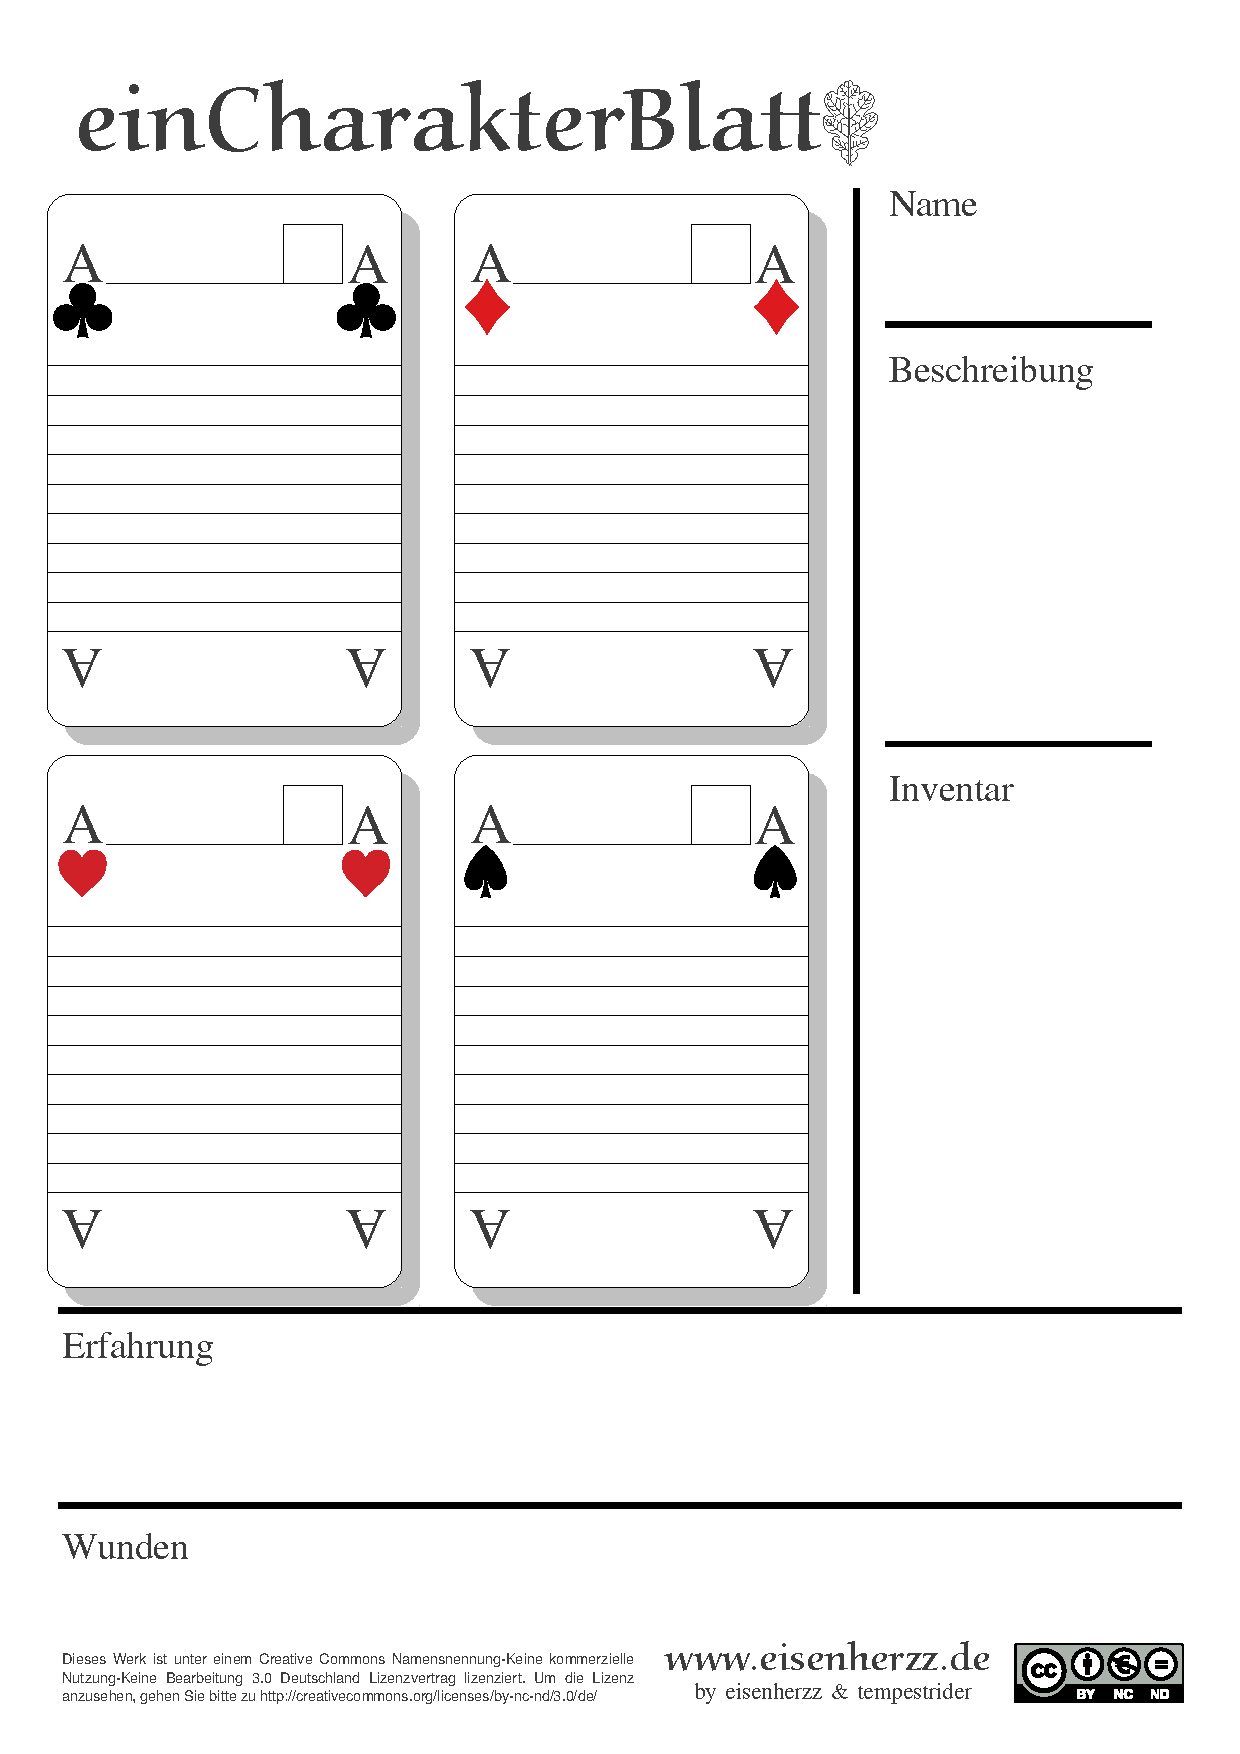
\includepdf[pages=1]{einCharakterBlatt/einCharakterBlatt.pdf}

\end{document}
